\documentclass[10pt,a4paper]{article}
\usepackage[utf8]{inputenc}
\usepackage[english]{babel}
\usepackage[T1]{fontenc}
\usepackage{amsmath}
\usepackage{amsfonts}
\usepackage{amssymb}
\usepackage{subcaption}
\usepackage{makeidx}
\usepackage{graphicx}
\usepackage{fourier}
\usepackage{listings}
\usepackage{color}
\usepackage{hyperref}
\usepackage[left=2cm,right=2cm,top=2cm,bottom=2cm]{geometry}
\author{Sigve Harang, Lukas Powalla}
\title{Space Physics Project , FYS3610}
\graphicspath{{./data/}} %BEEEEE CAREFUL WITH THIS LINE
\lstset{language=C++,
	keywordstyle=\bfseries\color{blue},
	commentstyle=\itshape\color{red},
	stringstyle=\color{green},
	identifierstyle=\bfseries,
	frame=single}
\begin{document}
\maketitle
\newpage
\tableofcontents
\newpage
\section*{Introduction}
In this project we are going to analyse the ionospheric and auroral dynamics and its relation to the solar wind conditions. Furthermore, we will connect our observations to the current systems as well as the auroral activity and polar cap.  We will investigate in a specific timeslot of 6 hours.  
\section{Theory part}
In order to understand the movements and changes in the system of the earth and the sun, we want to introduce some basic concepts of space physics. 
A really important steady state picture of what is going on with respect to the earth's magnetic field, the interaction of the earth's magnetic field with the IMF and the consequences of the earth's environment (such as current flows or aurora) is the Dungey cycle. (only when IMF is southward orientated)
However, the dungey cycle is as already mentioned a steady state picture. (This means for example that the magnetic flux added to the open magnetic field lines through day side reconnection is equal to the magnetic flux subtracting from the open magnetic field lines through night side reconnection)
However, this cycle is in reality not a steady state picture. There are different phases of adding magnetic flux (growing of the polar cap), some kind of explosive expansion (subtraction of magnetic flux from the polar cap) and a recovery phase. This phenomena is called a "Auroral substorm". In addition to that, we can extract information about what is going on with the system earth-sun by looking at different data sets containing information about the magnetic field on earth, the solar wind bulk speed, the auroral intensity, the current density and further data from different physical measurements. 
Based on this measurements we will interpret the received data and relate it to the theoretical predictions and the models we introduced in the theoretical part.

\subsection{The Dungey cycle - a steady state picture \label{Dungey cycle}}

\begin{figure}[h]
\centering
\caption{Dungey cycle}
\label{aurora substorm}
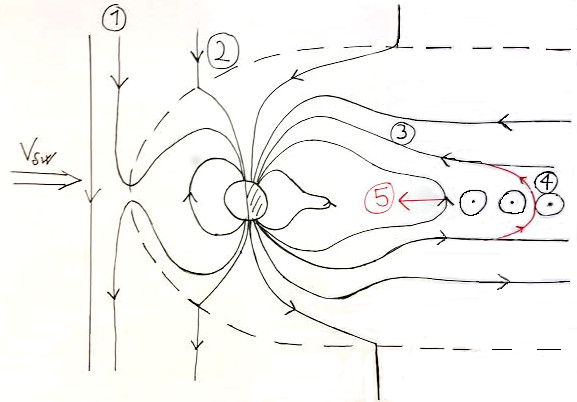
\includegraphics[scale=0.5]{solvind.jpg}
\end{figure}

If the magnetic field is northward orientated ($B_z>0$) nothing happens at the boundary of the terrestrial magnetic field and the magnetic field of the sun/ the solar wind. IMF can not mix with the terrestrial magnetic field because everything in frozen in. Since the terrestrial magnetic field and the IMF are not anti-parallel orientated, magnetic reconnection does not occur and hence, everything is and stays frozen in. 
However, if the IMF is southward orientated ($B_z<0$), we do have anti-parallel orientated magnetic field at the boundary of terrestrial magnetic field and the IMF (at the magnetopause). Therefore, magnetic reconnection occurs at the magnetopause, which causes a cyclic reconnection pattern at day/night-side. If we assume a steady state picture, we call the cycle, which happens for southward IMF, the dungey cycle. The different parts of the cycle can be described as follows:
\begin{itemize}
\item[1] opposite polarity field lines reconnect at magnetopause (if IMF southward orientated
\item[2] magnetic field lines are still connected to the solar wind. (frozen in again) Therefore, the magnetic field line is draged along with the solar wind in the direction of the tale. (magnetic tension force)
\item[3] magnetic flux is added to the tail and compresses the plasma sheet (magnetic pressure increases, plasma sheet gets thinner and thinner)
\item[4] magnetic reconnection occurs in the tail. 
\item[5] reconnected magnetic field lines return to the day side (imagination of "rubber bands" help to understand this)
\end{itemize}

\subsection{Auroral substorm}
As already mentioned in the introduction, the assumption of a steady state picture is not a appropriate description of what happens in reality. To specify this, the rate of adding magnetic flux and the rate of subtracting magnetic flux from the polar cap are not equal. However, after studying data from different measurements, Akasofu could state out in 1964 different phases of a cycle so called:
\begin{itemize}
\item[1] groth phase
\item[2] expansion phase
\item[3] recovery phase
\end{itemize}
\subsubsection{groth phase}
The day side reconnection dominates and the aurora moves to lower latitudes. The auroral activity increases in the cusp and open magnetic flux is added to the polar cap. The magnetic flux, which is added due to the day side reconnection makes the tail radius increase.(because the field lines are draged tail-wards with the IMF )
\subsubsection{Expansion phase}
Sudden onset of night-side reconnection at the NENL. Sudden brightening of the night side aurora. Poleward and westward movement of the aurora (on average). It closes open magnetic flux. 
\subsubsection{recovery phase}
The night side reconnection continues at smaller rates and the auroral display quietens. Furthermore, the polar cap contracts and the magnetosphere returns to pro groth phase "equilibrium". 
\begin{figure}[h]
\centering
\caption{Auroral substorm}
\label{aurora substorm}
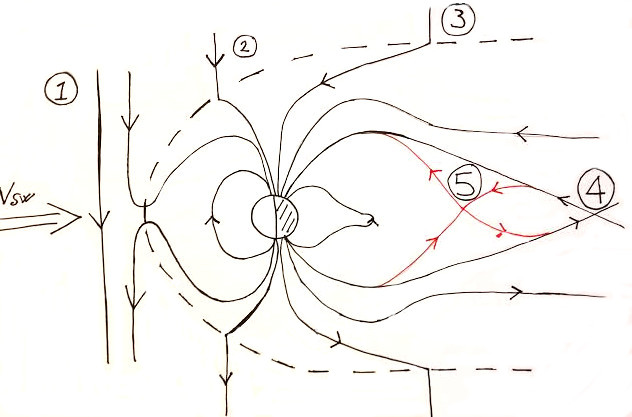
\includegraphics[scale=0.5]{solvind2.jpg}
\end{figure}

\subsection{currents}
In general, we can express the current flow in a given system with given magnetic field and electric field as follows:
\begin{align}
\vec{j}&= e n ( \vec{v}_i - \vec{v}_e ) = \sigma_p \vec{E}'_{\perp} + \sigma_H \frac{\vec{E}'_{\perp} \times \vec{B}}{B} + \sigma_{\parallel} \vec{E}_{\parallel}
\end{align}
Here, $\sigma_p$ is the Pedersen conductivity, $\sigma_H$ is the Hall conductivity and $\sigma_{\parallel}$ is a conductivity, which belongs to a current parallel to the electric field. We notice that the different currents caused by different conductivities flow in orthogonal directions with respect to each other. The orientation of $\vec{E}$ means parallel or orthogonal to the magnetic field. A discrete expression of the conductivities will not be needed in this report. 
\begin{align}
\vec{E}&= \vec{E}_{\perp} +\vec{E}_{\parallel}\\
\vec{E}'_{\perp}&=\vec{E}_{\perp}+ \vec{v}_n \times \vec{B}\\
\vec{E}'_{\perp}& \approx \vec{E}_{\perp}
\end{align}
The Electron Hall currents flow at lower altitudes than the Pedersen currents. 
The ionospheric Pedersen currents are connected to the Field aligned currents (FAC). The FAC are on the one hand side closed with the magnetopause current and on the other hand side with the ring current. All current systems need to be closed, which is the case. 

\subsection{Twin cell convection}
If we look at the Dungey cycle ($B_z<0$), we can figure out the movement of the open/closed field lines at the polar caps, which gives us the movement of the particles at the polar cap. 
Let us first explain, what leads to the so called "Twin-cell"-convection. If we have southward IMF, the orientation of the IMF and the earth's magnetic field are opposite to each other. Like discussed in chapter \ref{Dungey cycle}, magnetic reconnection on the day side of the earth can occur. The magnetic reconnection at the day side adds open magnetic field lines to the polar cap. In other words, day side reconnection adds magnetic flux to the polar cap. 
The deformation of the usually round open/closed-field boundary leads to a movement, which tries to "smooth out" the little bump in the boundary. Magnetic field lines naturally want themselves to orientate in a straight line. 

Let us now look at the night side. If we look at the night side events, we know that magnetic reconnection occurs in the tail.(dungey cycle) Reasons for this happening are for example that through day side reconnection, magnetic flux is added to the tail, the magnetic pressure increases and leads in the end to magnetic reconnection in the tail. 
The magnetic reconnection to the tail closes open magnetic field lines. This means that the polar cap shrinks a bit on the night side. In other words, magnetic flux is subtracted at the night side of the earth from the polar cap. The subtraction leads to a little dint in the polar cap. The magnetic field lines tend to "smooth out" the little dint, which leads to a corresponding movement. 

In total, we expect now a movement, which is well known as the twin cell convection. The electric potential on the poles will give us the movement of the charged particles. The currents move along potential lines. The equipotential lines are therefore the trajectories of the charged particles. The currents are called "Hall"-currents. The hall-currents can be found in an altitude of approximately 110 km. (electro-jets)
\subsection{Earth- Corotation and Dungey-cycle}


\section{Observations}

All in all, we use five different sources and data to draw an image of what is going on with the interaction of the IMF with the earth's magnetic field. 
First of all, we use a satellite called ACE (Advanced composition explorer) in order to get knowledge about the magnetic field of the IMF at earth's position. The ACE satellite orbits the Lagrangian point $L_1$. This Lagrangian point sits exactly between the earth and the sun. The solar wind particles move radially outwards from the sun. Therefore, the data from ACE can be used to describe the IMF at earth's position when we take the time into account, which is needed from the solar wind to travel from the position of the ACE to earth. 
If we take a look at the position of ACE and the solar-wind speed at the position of ACE, we can calculate the time the IMF needs to travel from ACE to earth. 
Finally, we know what the IMF looks like at earth's position at a given time on earth. 
This is important because we know from the chapter \ref{Dungey cycle}, that the $B_z$ tells us something about magnetic reconnection on the day side. If $B_z>0$ (or northward IMF orientation), there is no magnetic reconnection on the day side. There is no open magnetic flux added to the polar cap. 
However, if the $Bz$ component is negative (or southward orientation of IMF) magnetic reconnection on the day side can occur and the dungey cycle kicks in. 
It is therefore very important to get data from the $B_z$ component of the IMF. The other components of the IMF can be used at a later point to tell something about the specific shape of the twin-cell convection. 


\subsection{ACE}
In this section, we want to discuss the data from the ACE. In figures \ref{ACE Solarwindspeed} and \ref{ACE distance}, we find data from the solarwindspeed and the ACE position. Both together will be used to determine the time delay of the IMF. The coordinate system GSE (Geocentric Solar Ecliptic). If we assume a average velocity of the solar wind (see \ref{ACE Solarwindspeed} $V_x$) of $400 \frac{m}{s}$ and a average distance of $1.4802 \cdot 10^{6} \mathrm{km}$ from ACE to earth, we get a average time delay of 1 hour and $1.7$ minutes. This is the time, the solar wind needs to travel from ACE to earth. 

\begin{figure}[h]
\centering
\begin{subfigure}{0.45\textwidth}
\centering
	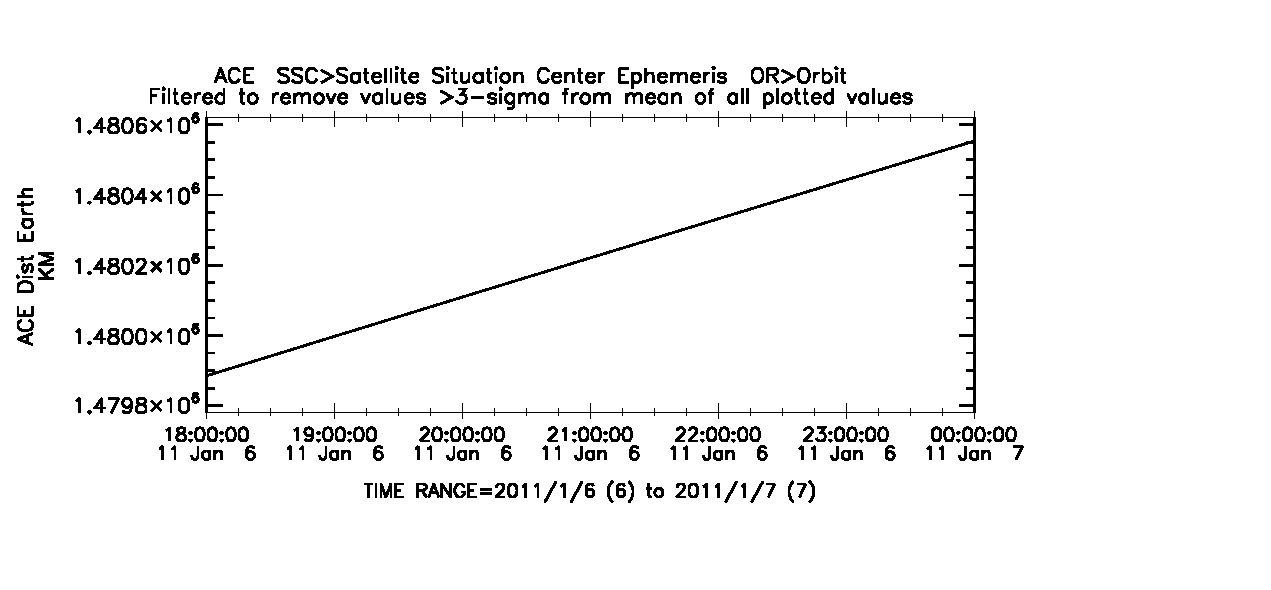
\includegraphics[width=\textwidth]{ACE_distance.pdf}
	\caption{ ACE distance from earth \label{ACE distance}}
\end{subfigure}
\begin{subfigure}{0.45\textwidth}
\centering
	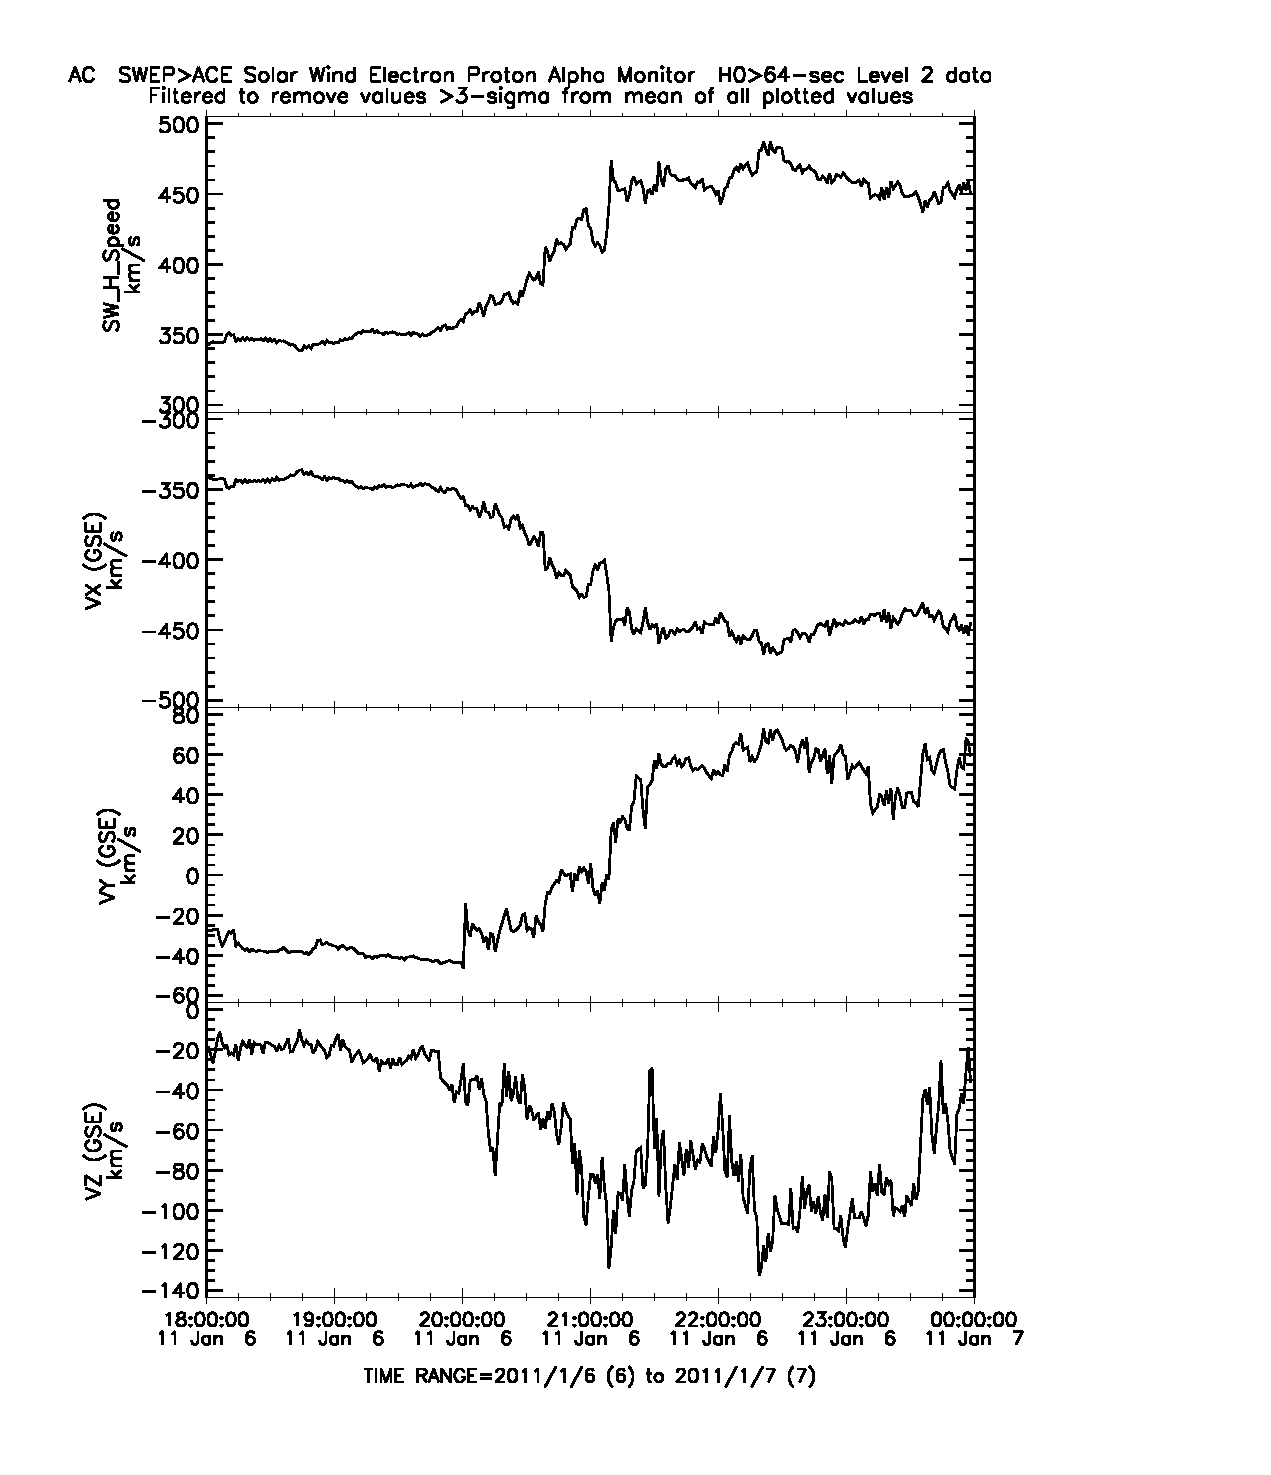
\includegraphics[width=\textwidth]{ACE_solarwindspeed.pdf}
	\caption{ Solarwind data\label{ACE Solarwindspeed}}
\end{subfigure}
\caption{ACE data}
\end{figure}

\begin{figure}
\centering
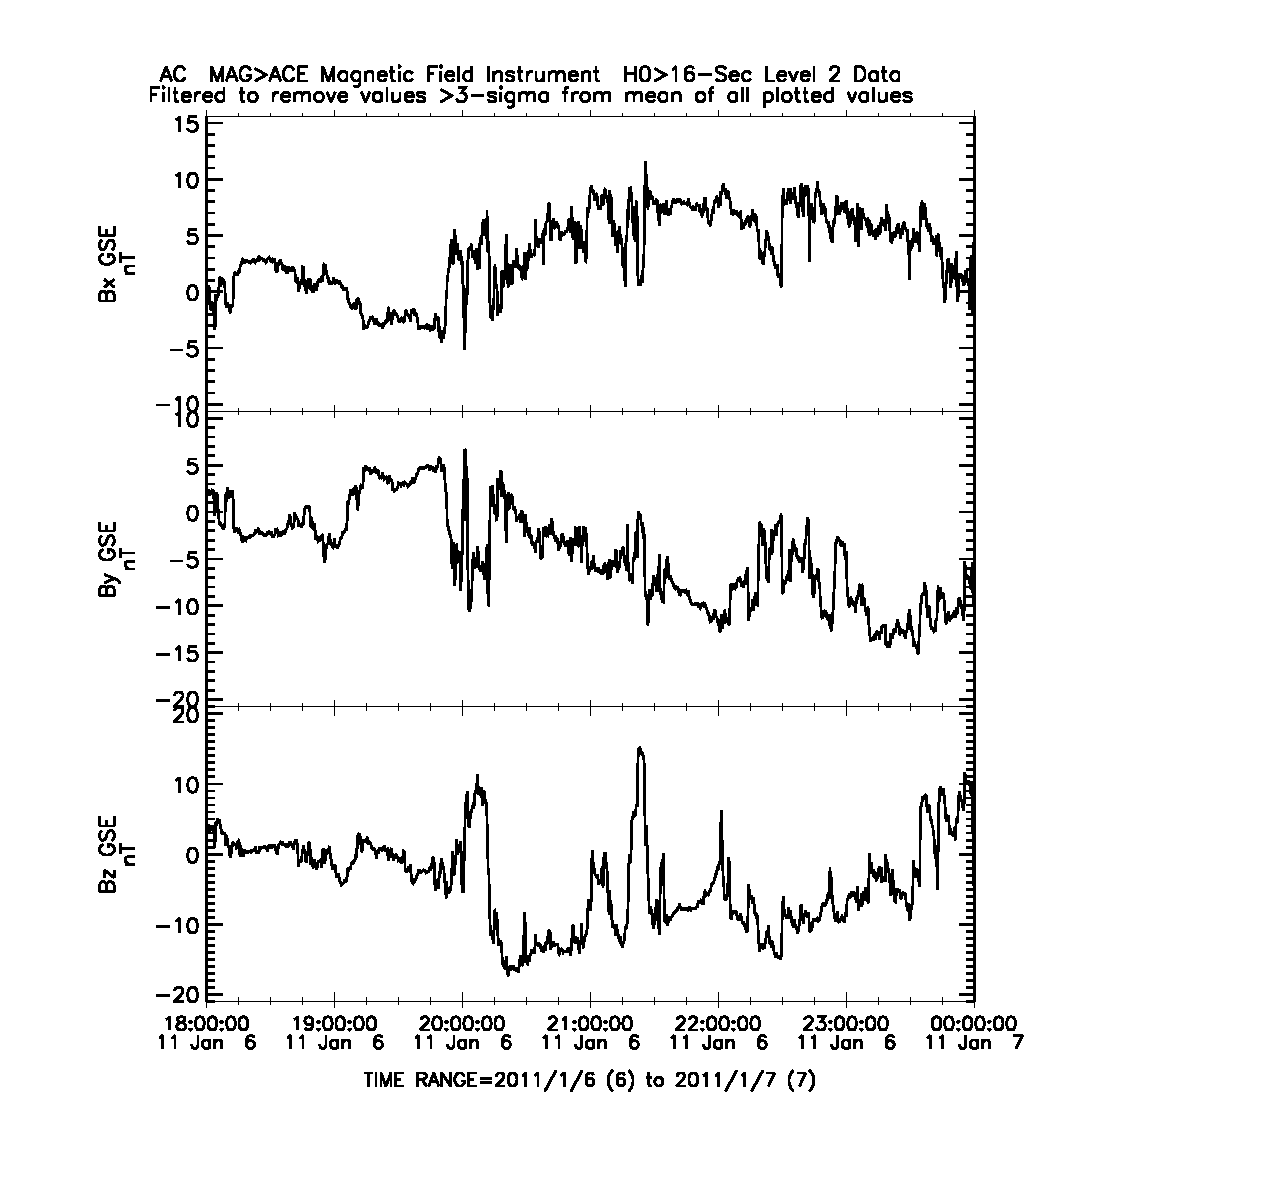
\includegraphics[width=0.6\textwidth]{ACE_magneticfield.pdf}
\caption{magnetic field measured at the ACE}
\end{figure}


\subsection{AMPERE}


\begin{figure}[h]
\centering
\begin{subfigure}{0.3\textwidth}
\centering
	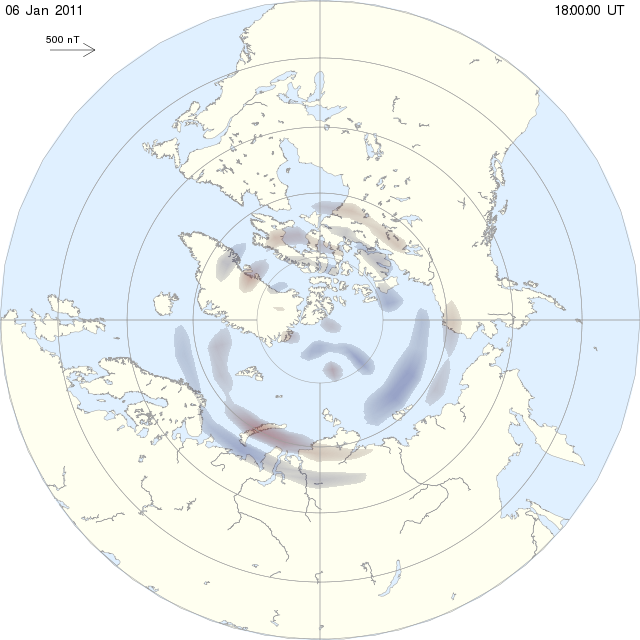
\includegraphics[width=\textwidth]{ampere0.png}
	\caption{ 18:00 o'clock\label{amp18}}
\end{subfigure}
\begin{subfigure}{0.3\textwidth}
\centering
	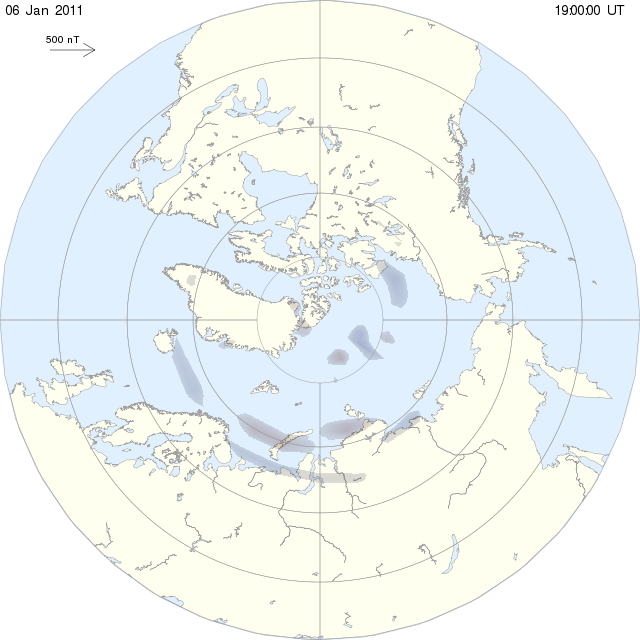
\includegraphics[width=\textwidth]{ampere1.png}
	\caption{19:00 o'clock \label{amp19}}
\end{subfigure}
\begin{subfigure}{0.3\textwidth}
\centering
	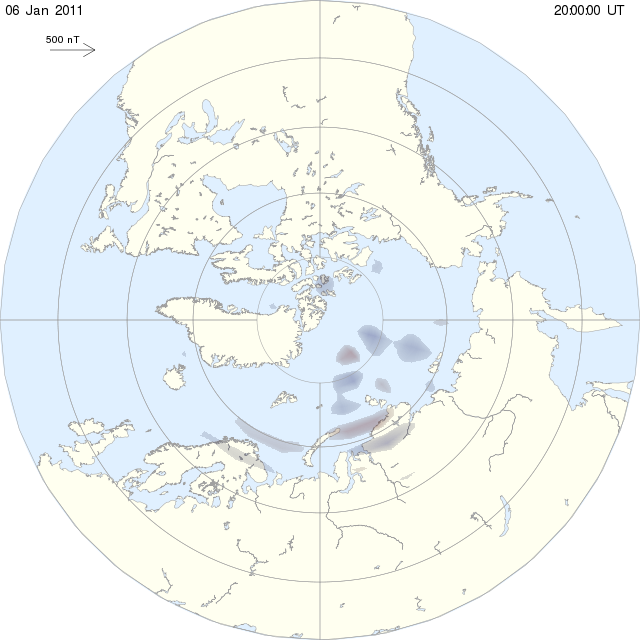
\includegraphics[width=\textwidth]{ampere2.png}
	\caption{ 20:00 o'clock \label{amp20}}
\end{subfigure}
\begin{subfigure}{0.3\textwidth}
\centering
	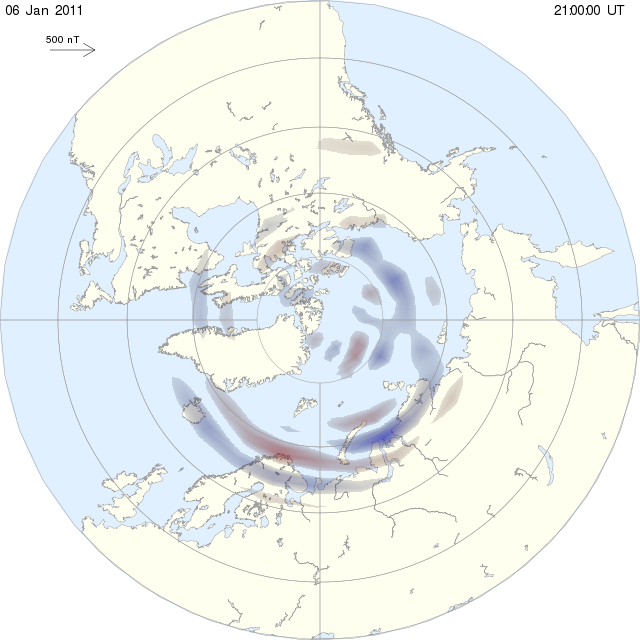
\includegraphics[width=\textwidth]{ampere3.png}
	\caption{ 21:00 o'clock \label{amp21}}
\end{subfigure}
\begin{subfigure}{0.3\textwidth}
\centering
	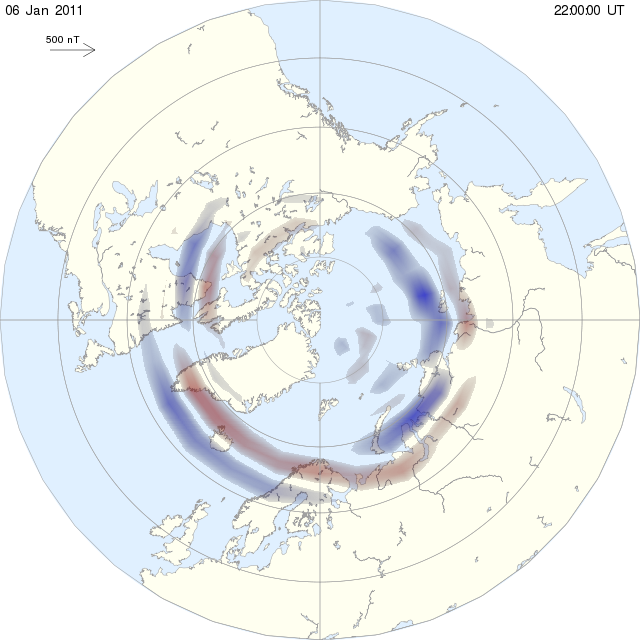
\includegraphics[width=\textwidth]{ampere4.png}
	\caption{ 22:00 o'clock \label{amp22}}
\end{subfigure}
\begin{subfigure}{0.3\textwidth}
\centering
	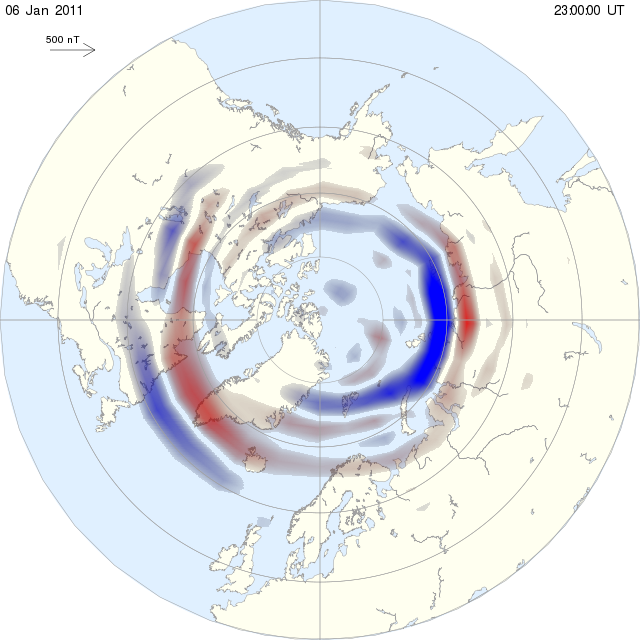
\includegraphics[width=\textwidth]{ampere5.png}
	\caption{ 23:00 o'clock \label{amp23}}
\end{subfigure}
\begin{subfigure}{0.3\textwidth}
\centering
	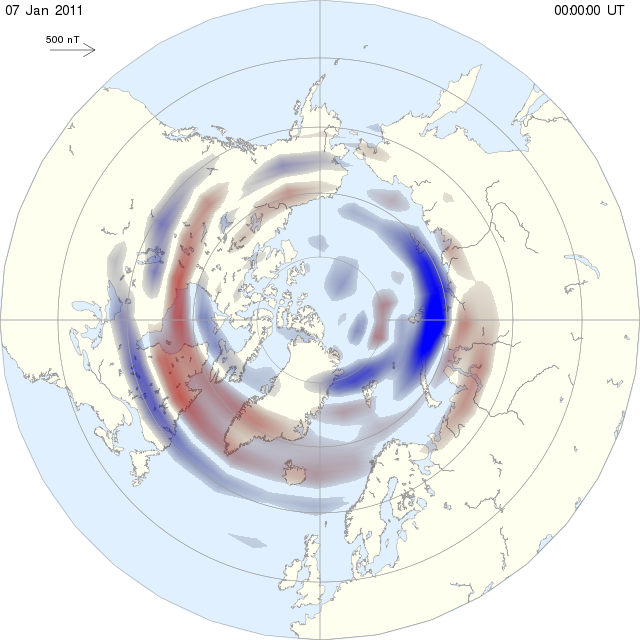
\includegraphics[width=\textwidth]{ampere6.png}
	\caption{ 00:00 o'clock (next day) \label{amp00}}
\end{subfigure}
\begin{subfigure}{0.3\textwidth}
\centering
	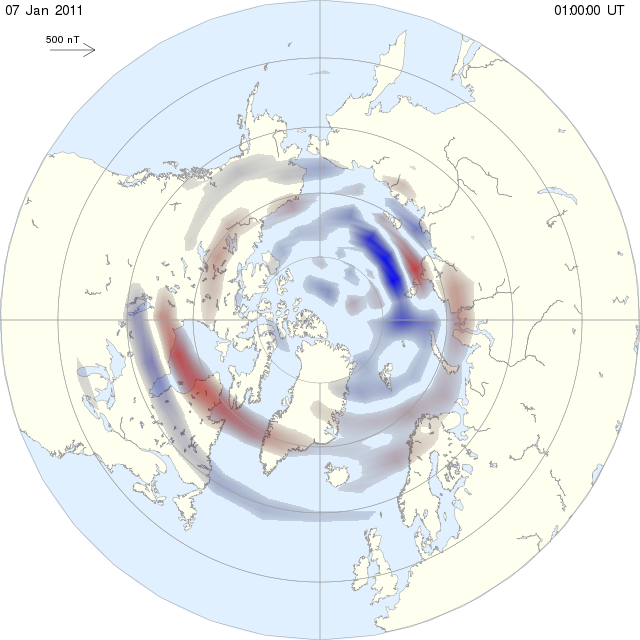
\includegraphics[width=\textwidth]{ampere7.png}
	\caption{ 01:00 o'clock \label{amp01}}
\end{subfigure}
\begin{subfigure}{0.3\textwidth}
\centering
	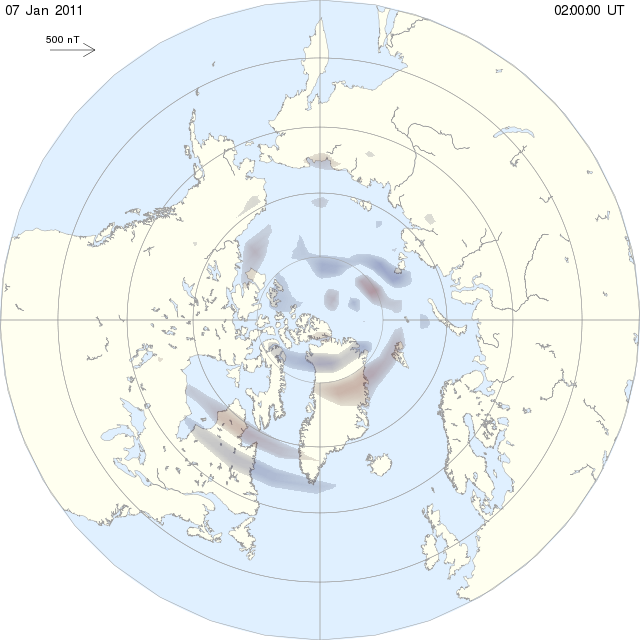
\includegraphics[width=\textwidth]{ampere8.png}
	\caption{ 02:00 o'clock \label{amp02}}
\end{subfigure}
\caption{Data from AMPERE at different times}
\end{figure}



\subsection{Groundbasedmagnetometer}

\begin{figure}[h]
\centering
\begin{subfigure}{0.3\textwidth}
\centering
	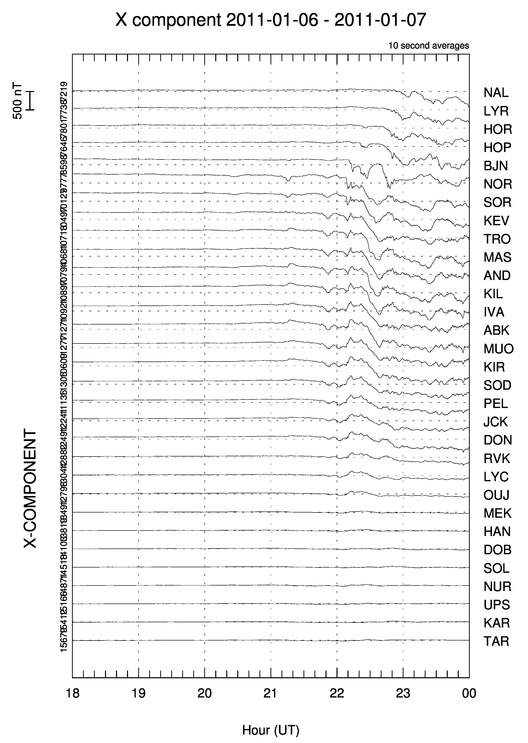
\includegraphics[width=\textwidth]{X_gram.jpg}
	\caption{ Groundbasedmagnetometer x-direction \label{GBM_X}}
\end{subfigure}
\begin{subfigure}{0.3\textwidth}
\centering
	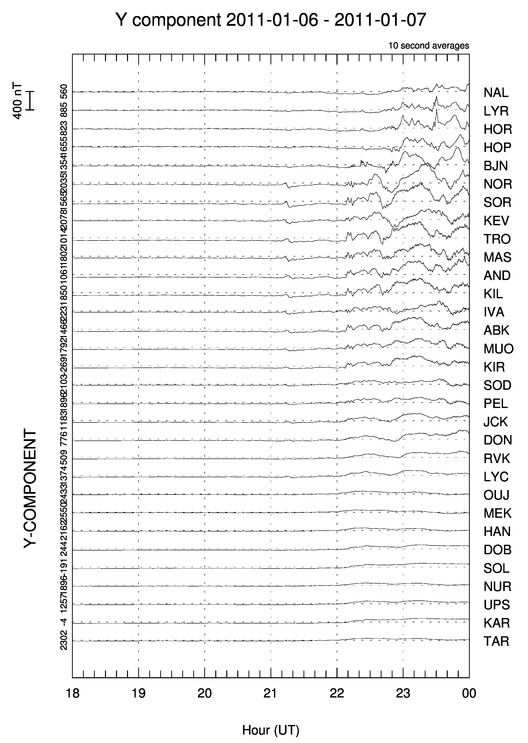
\includegraphics[width=\textwidth]{Y_gram.jpg}
	\caption{ Groundbasedmagnetometer y-direction \label{GBM_Y}}
\end{subfigure}
\begin{subfigure}{0.3\textwidth}
\centering
	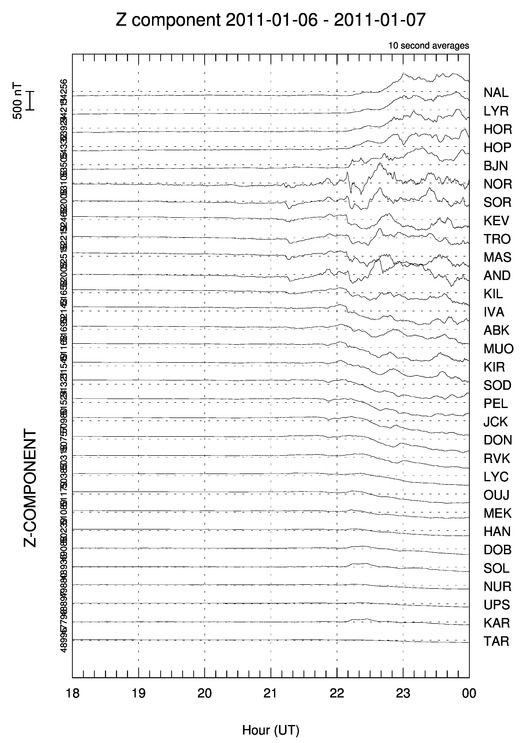
\includegraphics[width=\textwidth]{Z_gram.jpg}
	\caption{  Groundbasedmagnetometer z-direction\label{GBM_Z}}
\end{subfigure}
\caption{Data from Groundbasedmagnetometer, different components }
\end{figure}

\clearpage

\subsection{Superdarn}

\begin{figure}[h]
\centering
\begin{subfigure}{0.3\textwidth}
\centering
	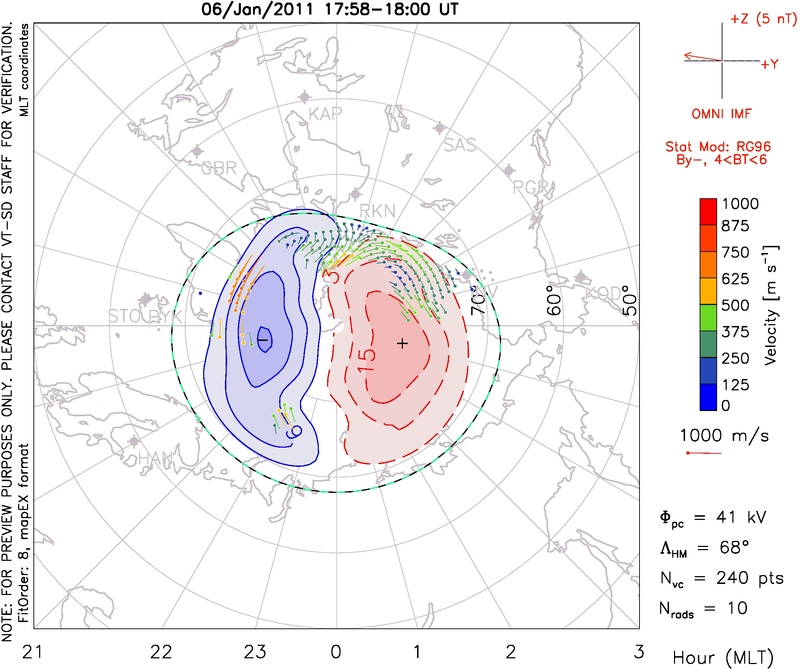
\includegraphics[width=\textwidth]{Superdarn1.jpg}
	\caption{ Superdarn at 18:00 o'clock \label{Super_18}}
\end{subfigure}
\begin{subfigure}{0.3\textwidth}
\centering
	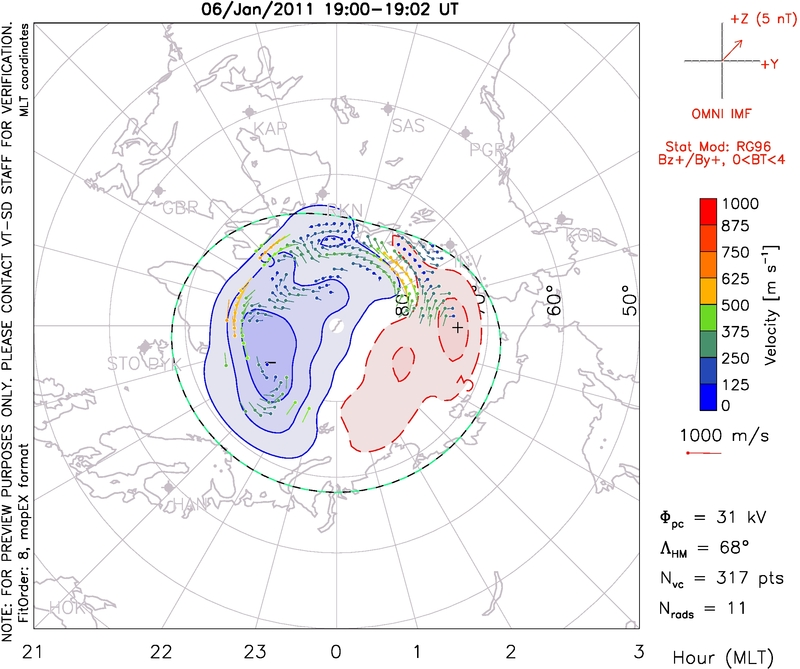
\includegraphics[width=\textwidth]{Superdarn2.jpg}
	\caption{ Superdarn at 19:00 o'clock \label{Super_19}}
\end{subfigure}
\begin{subfigure}{0.3\textwidth}
\centering
	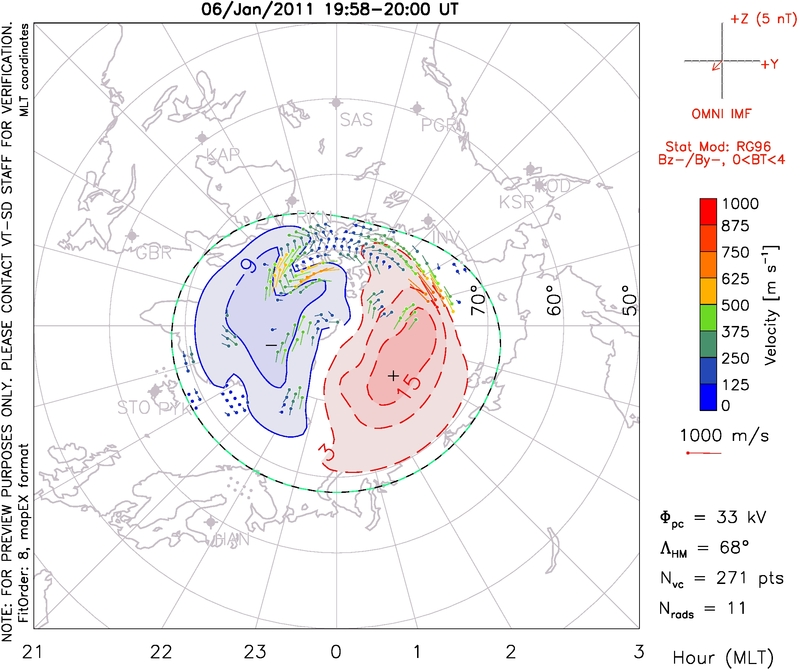
\includegraphics[width=\textwidth]{Superdarn3.jpg}
	\caption{ Superdarn at 20:00 o'clock \label{Super_20}}
\end{subfigure}
\begin{subfigure}{0.3\textwidth}
\centering
	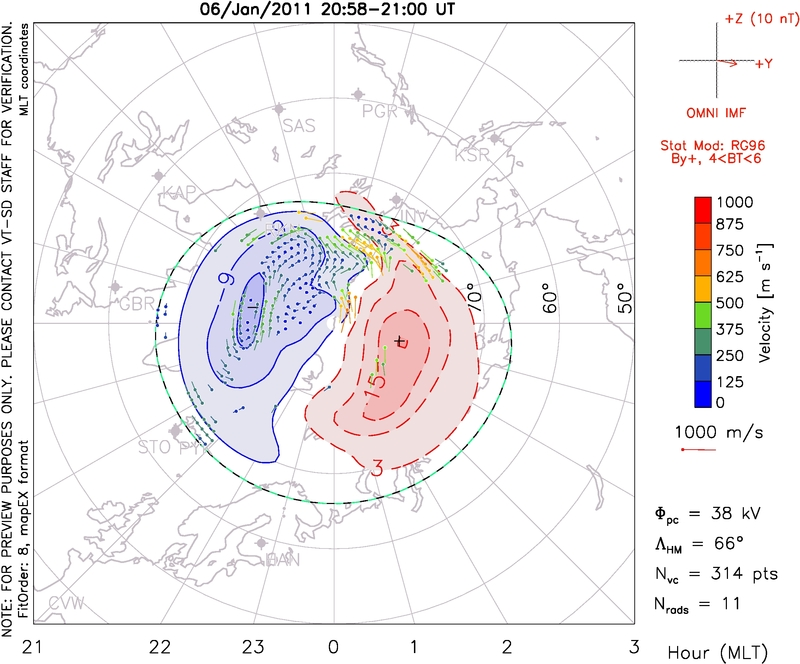
\includegraphics[width=\textwidth]{Superdarn4.jpg}
	\caption{ Superdarn at 21:00 o'clock \label{Super_21}}
\end{subfigure}
\begin{subfigure}{0.3\textwidth}
\centering
	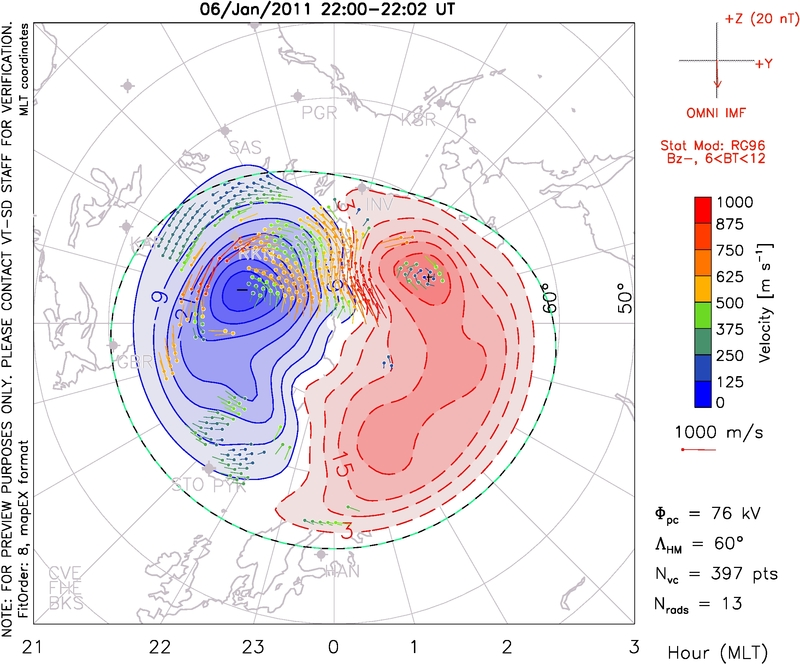
\includegraphics[width=\textwidth]{Superdarn5.jpg}
	\caption{ Superdarn at 22:00 o'clock \label{Super_22}}
\end{subfigure}
\begin{subfigure}{0.3\textwidth}
\centering
	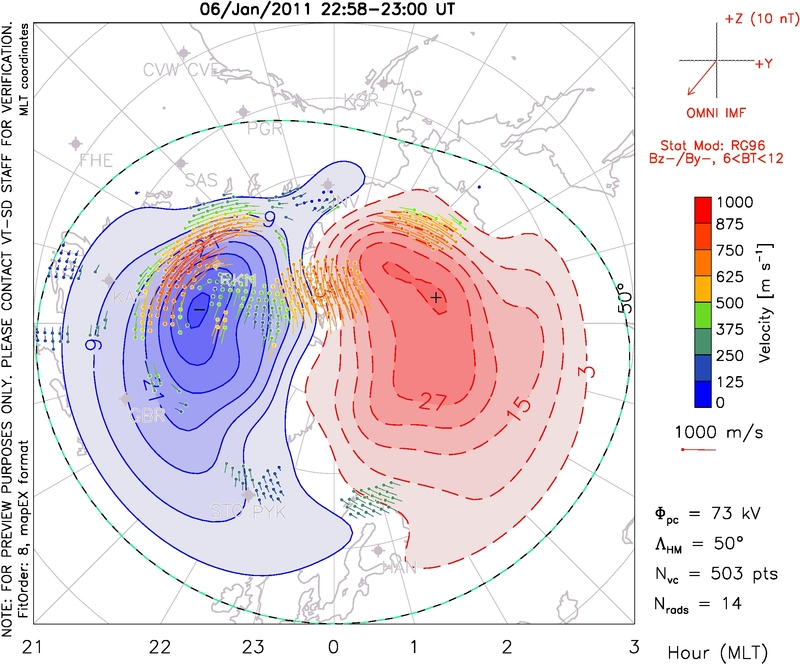
\includegraphics[width=\textwidth]{Superdarn6.jpg}
	\caption{ Superdarn at 23:00 o'clock \label{Super_23}}
\end{subfigure}
\begin{subfigure}{0.3\textwidth}
\centering
	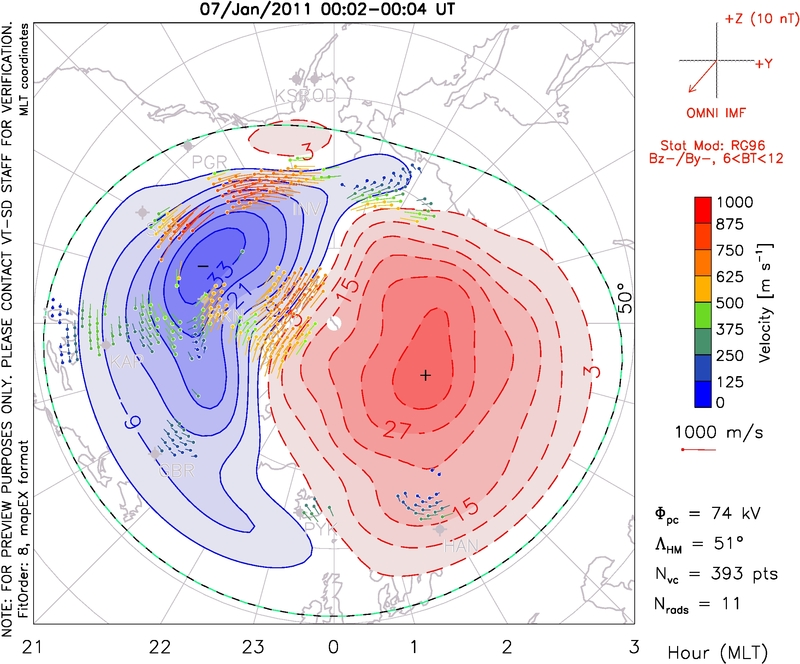
\includegraphics[width=\textwidth]{Superdarn7.jpg}
	\caption{ Superdarn at 00:00 o'clock, next day \label{Super_00}}
\end{subfigure}
\begin{subfigure}{0.3\textwidth}
\centering
	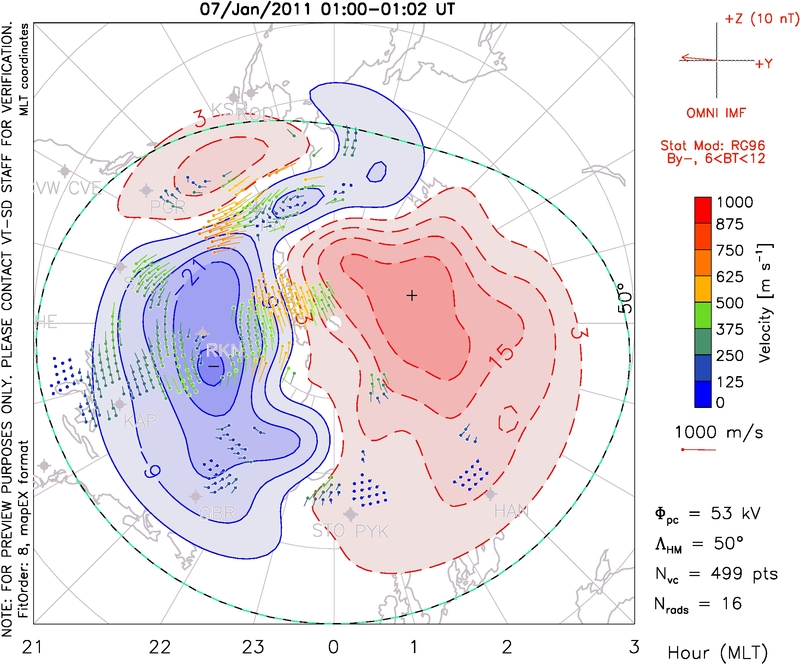
\includegraphics[width=\textwidth]{Superdarn8.jpg}
	\caption{ Superdarn at 01:00 o'clock \label{Super_01}}
\end{subfigure}
\begin{subfigure}{0.3\textwidth}
\centering
	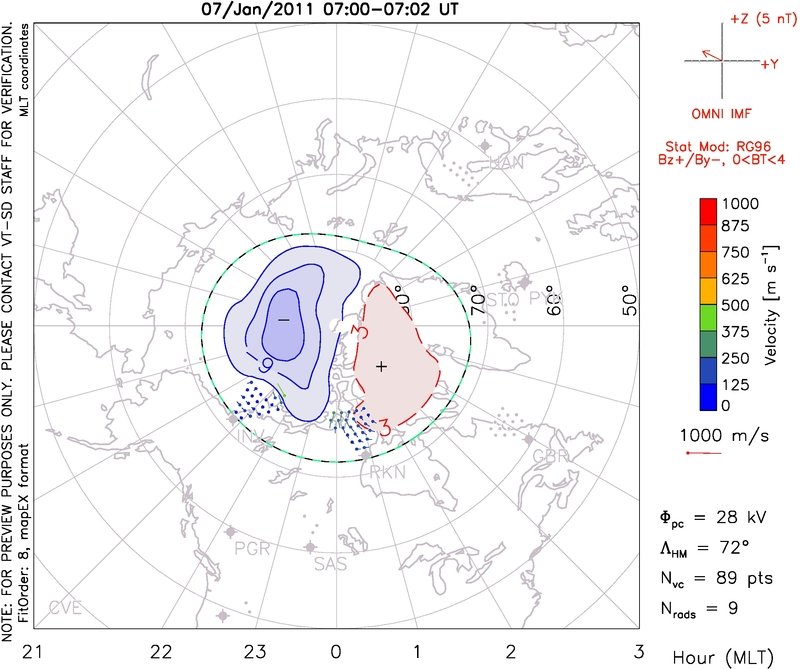
\includegraphics[width=\textwidth]{Superdarn14.jpg}
	\caption{ Superdarn at 07:00 o'clock \label{Super_07}}
\end{subfigure}
\caption{data from Superdarn for different times}
\end{figure}

\subsection{Svalbardimager}

\begin{figure}[h]
\centering
\begin{subfigure}{0.45\textwidth}
\centering
	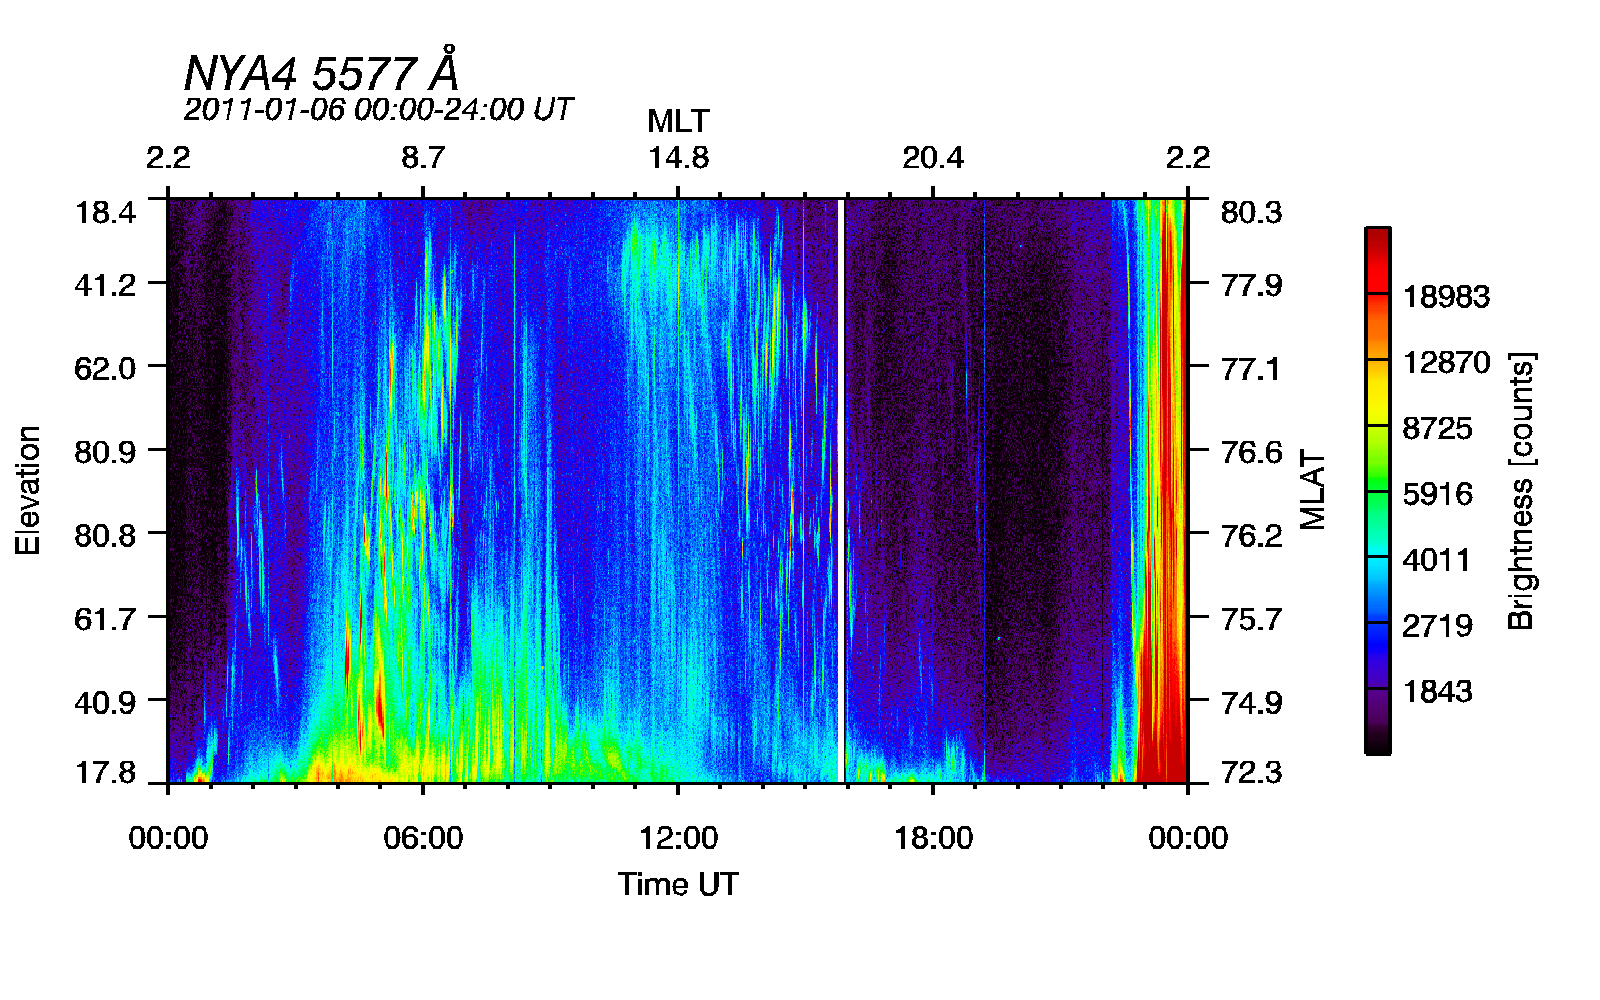
\includegraphics[width=\textwidth]{SvalbardImager5577A.png}
	\caption{ SvalbardImager for 5577 $\r{A}$ \label{SBI_5_overview}}
\end{subfigure}
\begin{subfigure}{0.45\textwidth}
\centering
	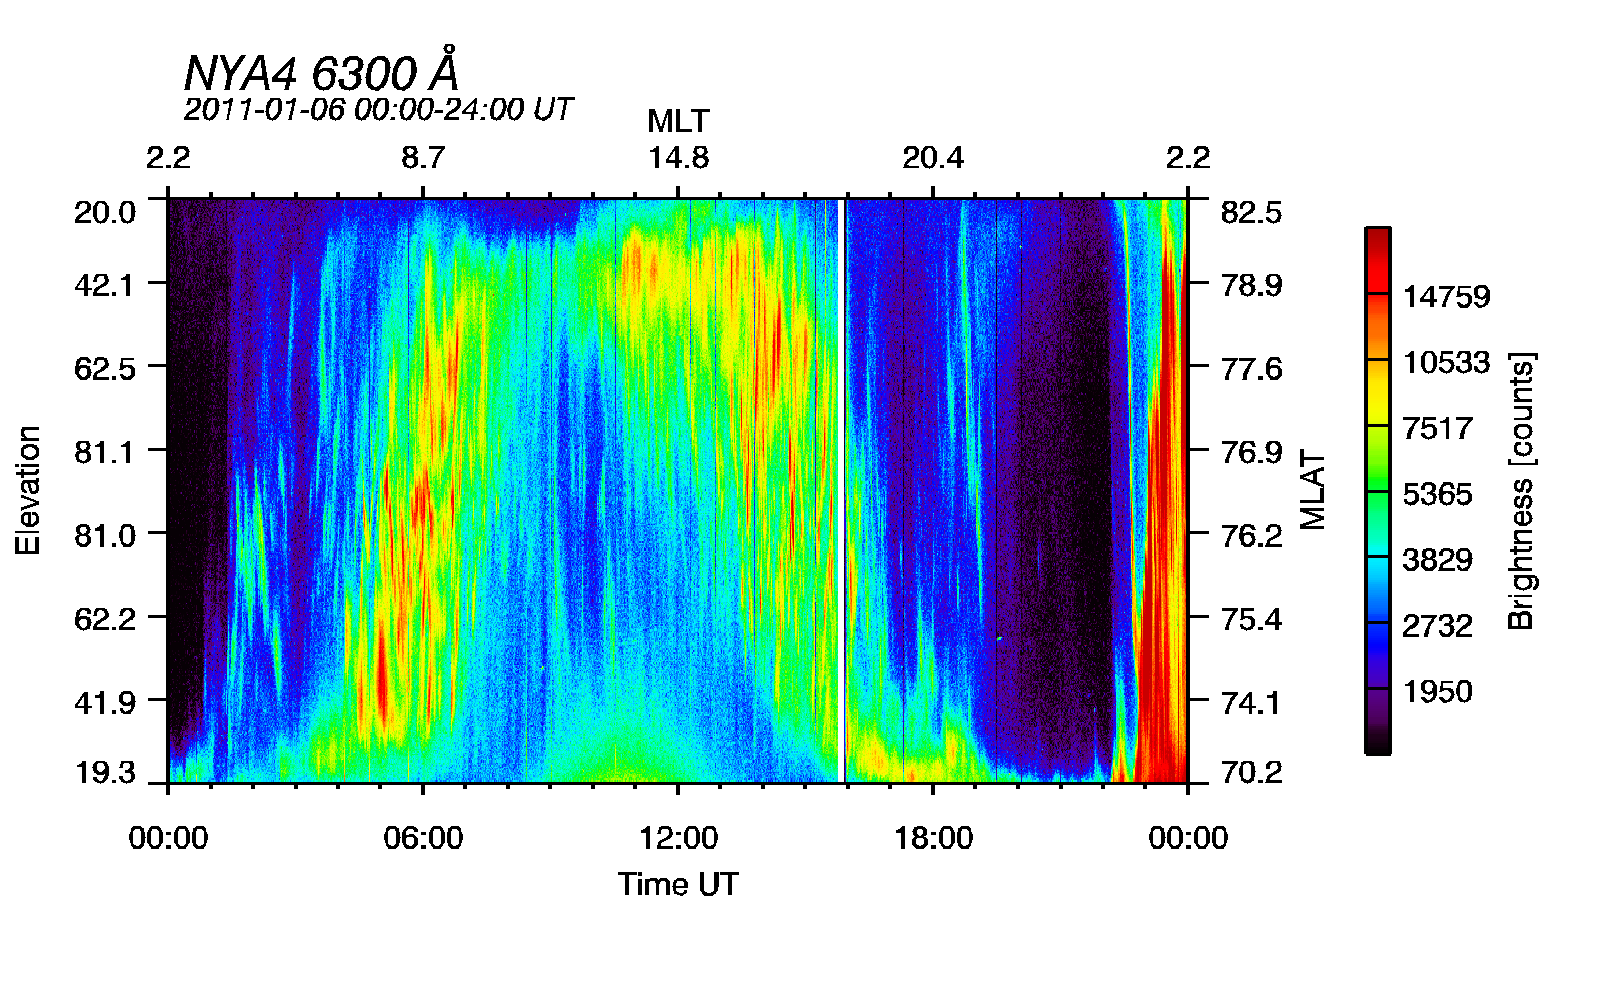
\includegraphics[width=\textwidth]{SvalbardImager6300A.png}
	\caption{ SvalbardImager for 6300 $\r{A}$\label{SBI_6_overview}}
\end{subfigure}
\caption{Overview over the Svalbard-Imagers}
\end{figure}

\begin{figure}[h]
\centering
\begin{subfigure}{0.3\textwidth}
\centering
	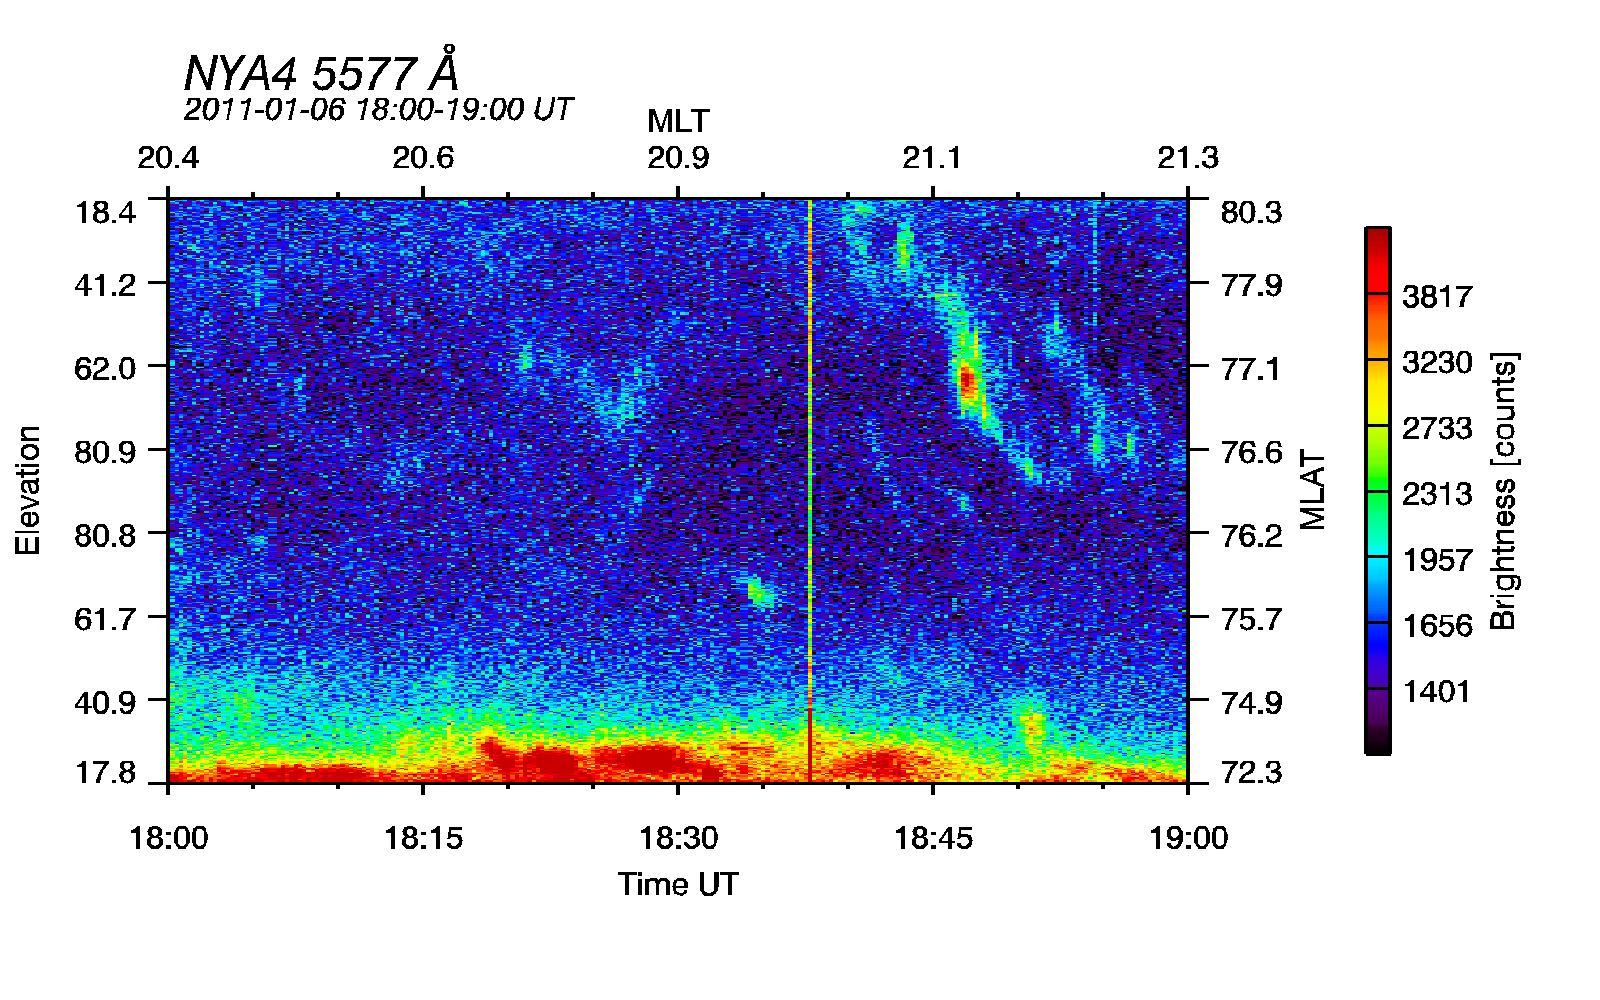
\includegraphics[width=\textwidth]{SvalbardImager5577A18.png}
	\caption{ SvalbardImager at 18:00 o'clock \label{SBI_5_18}}
\end{subfigure}
\begin{subfigure}{0.3\textwidth}
\centering
	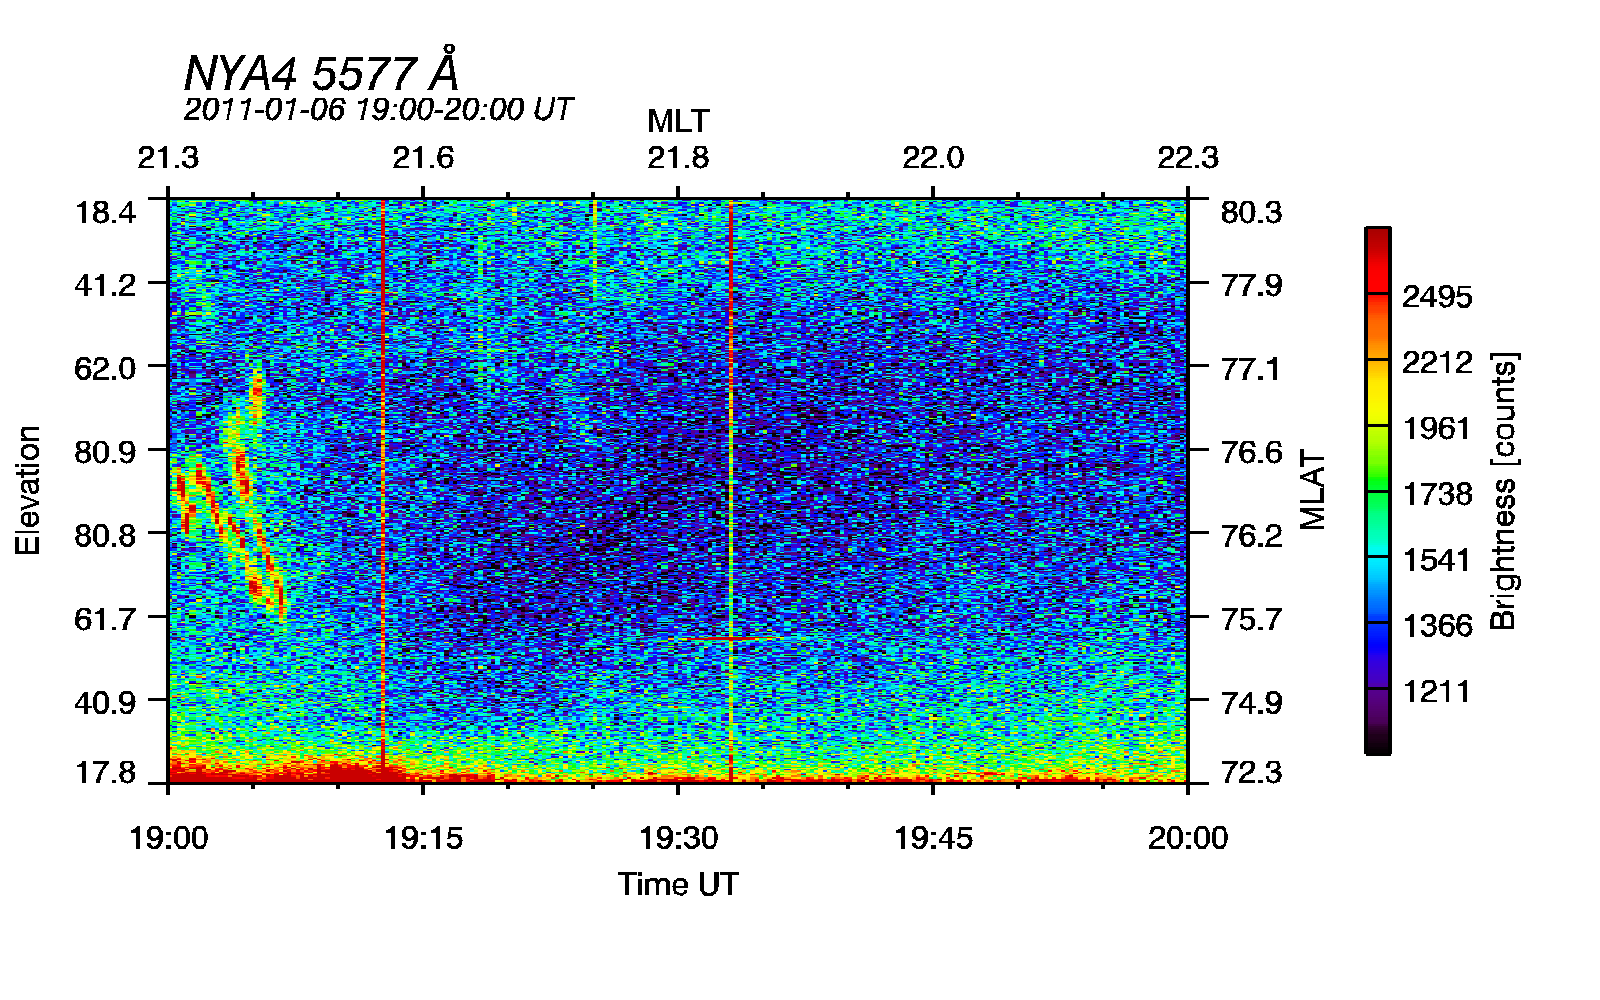
\includegraphics[width=\textwidth]{SvalbardImager5577A19.png}
	\caption{ SvalbardImager at 19:00 o'clock \label{SBI_5_19}}
\end{subfigure}
\begin{subfigure}{0.3\textwidth}
\centering
	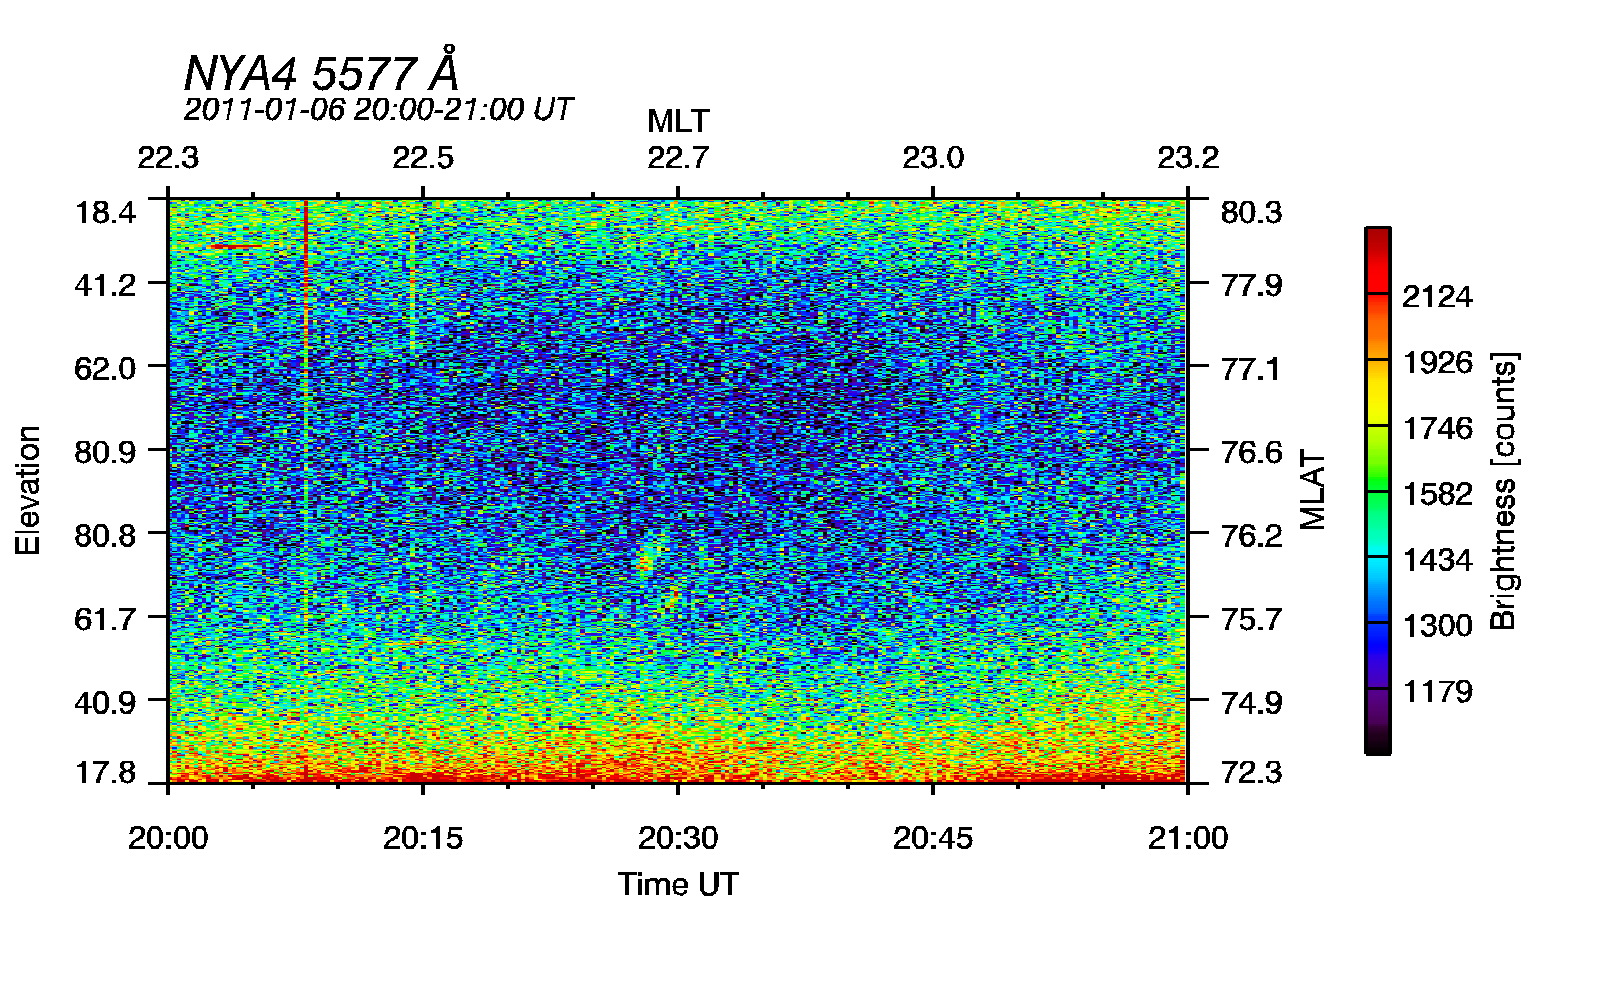
\includegraphics[width=\textwidth]{SvalbardImager5577A20.png}
	\caption{ SvalbardImager at 20:00 o'clock \label{SBI_5_20}}
\end{subfigure}
\begin{subfigure}{0.3\textwidth}
\centering
	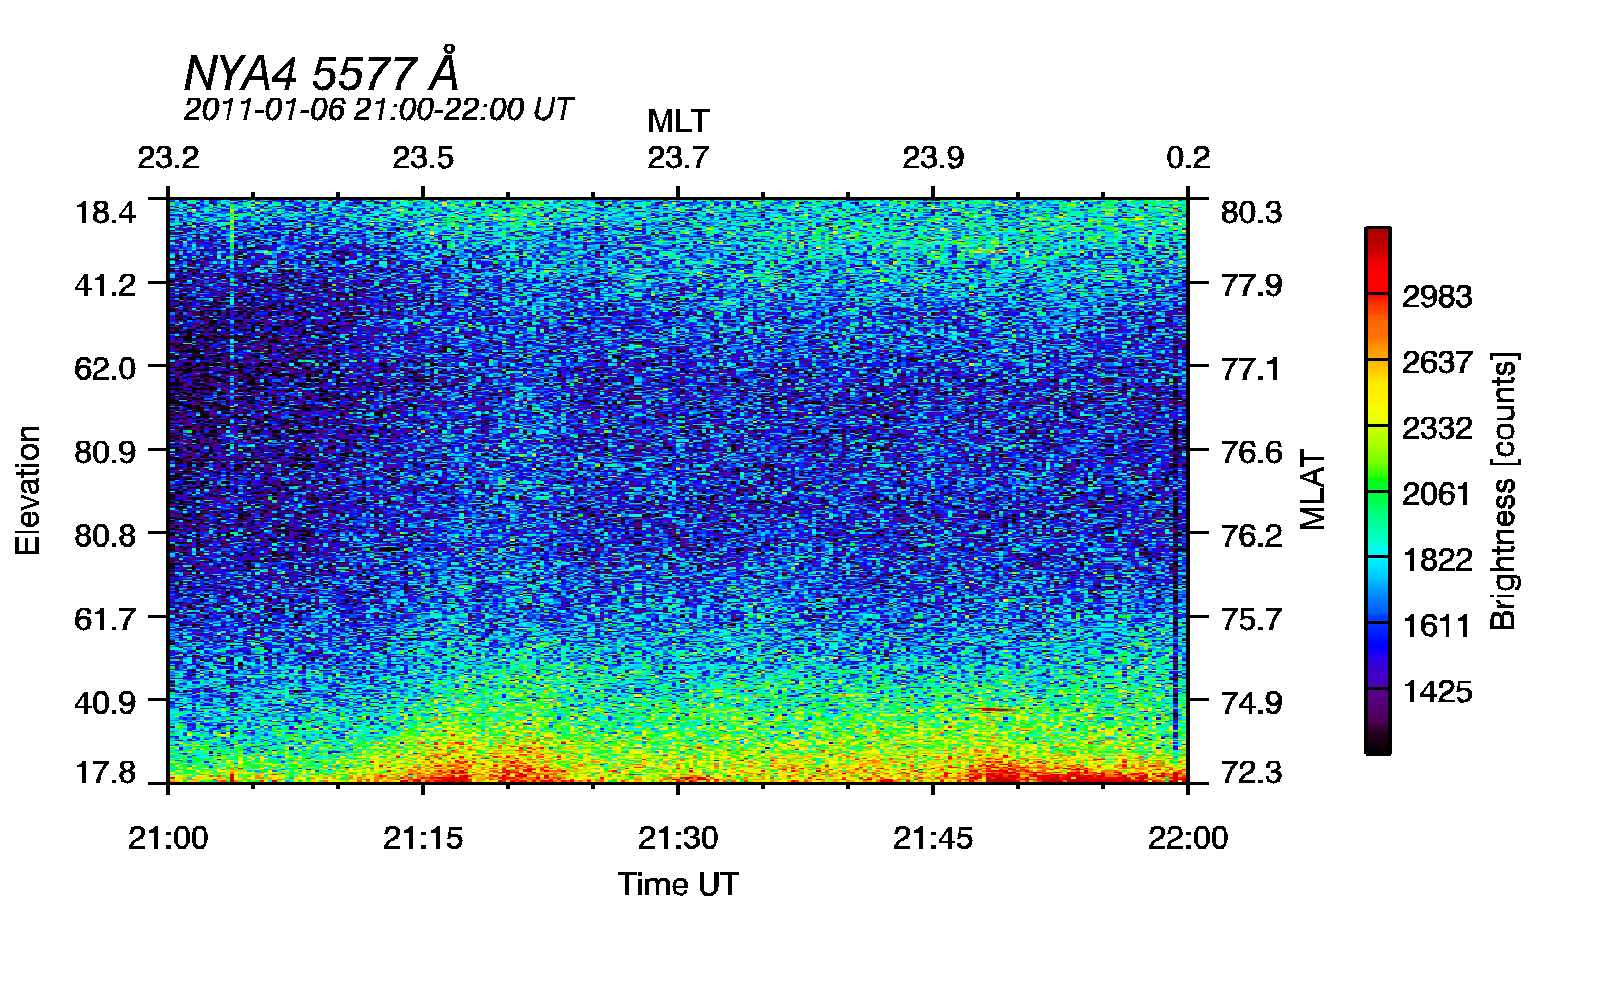
\includegraphics[width=\textwidth]{SvalbardImager5577A21.png}
	\caption{ SvalbardImager at 21:00 o'clock \label{SBI_5_21}}
\end{subfigure}
\begin{subfigure}{0.3\textwidth}
\centering
	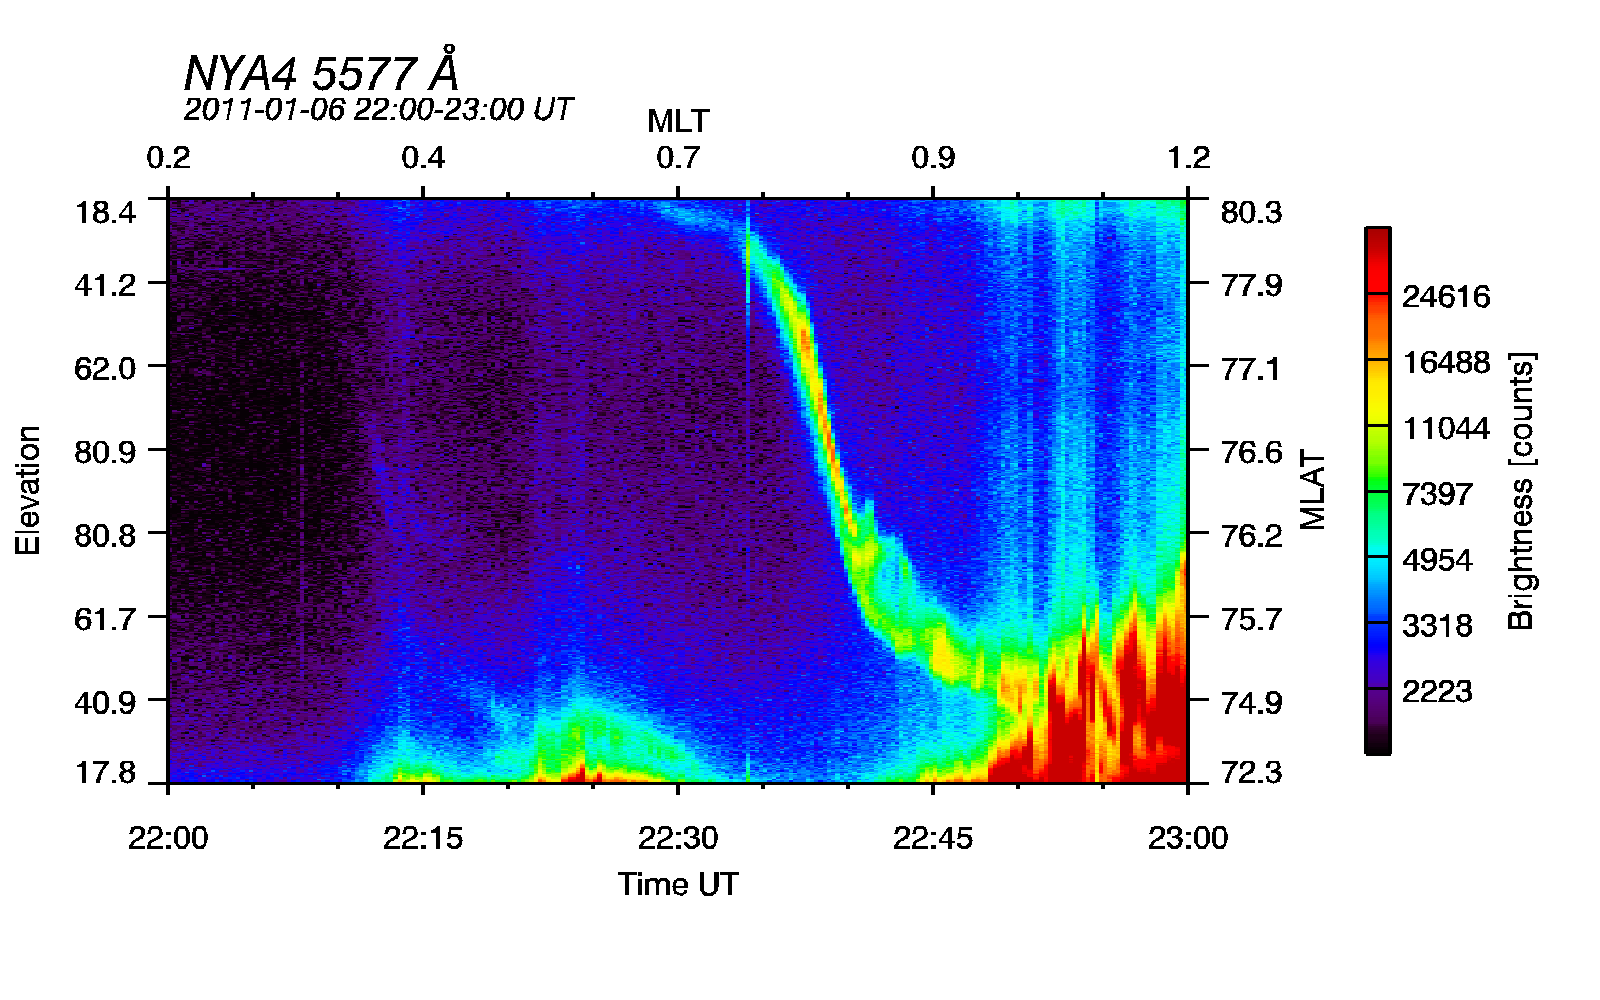
\includegraphics[width=\textwidth]{SvalbardImager5577A22.png}
	\caption{ SvalbardImager at 22:00 o'clock \label{SBI_5_22}}
\end{subfigure}
\begin{subfigure}{0.3\textwidth}
\centering
	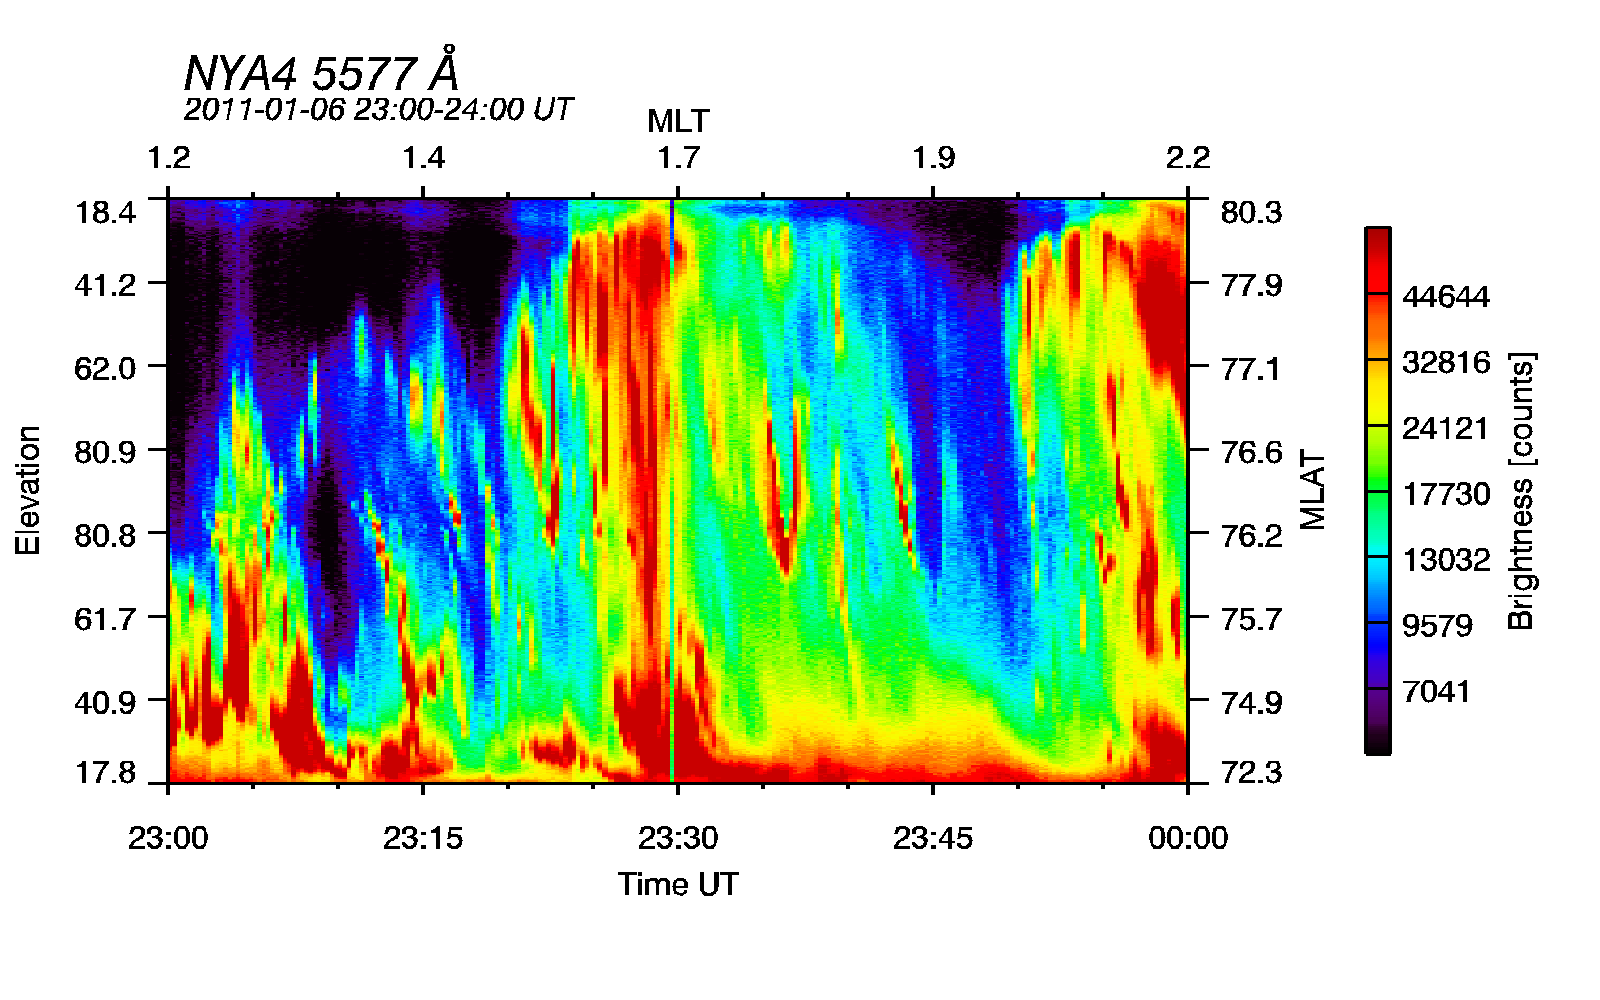
\includegraphics[width=\textwidth]{SvalbardImager5577A23.png}
	\caption{ SvalbardImager at 23:00 o'clock \label{SBI_5_23}}
\end{subfigure}
\caption{Ketograms from the SvalbardImager for $\lambda=5577 \cdot 10^{-10} \mathrm{m}$, different times }
\end{figure}

\begin{figure}[h]
\centering
\begin{subfigure}{0.3\textwidth}
\centering
	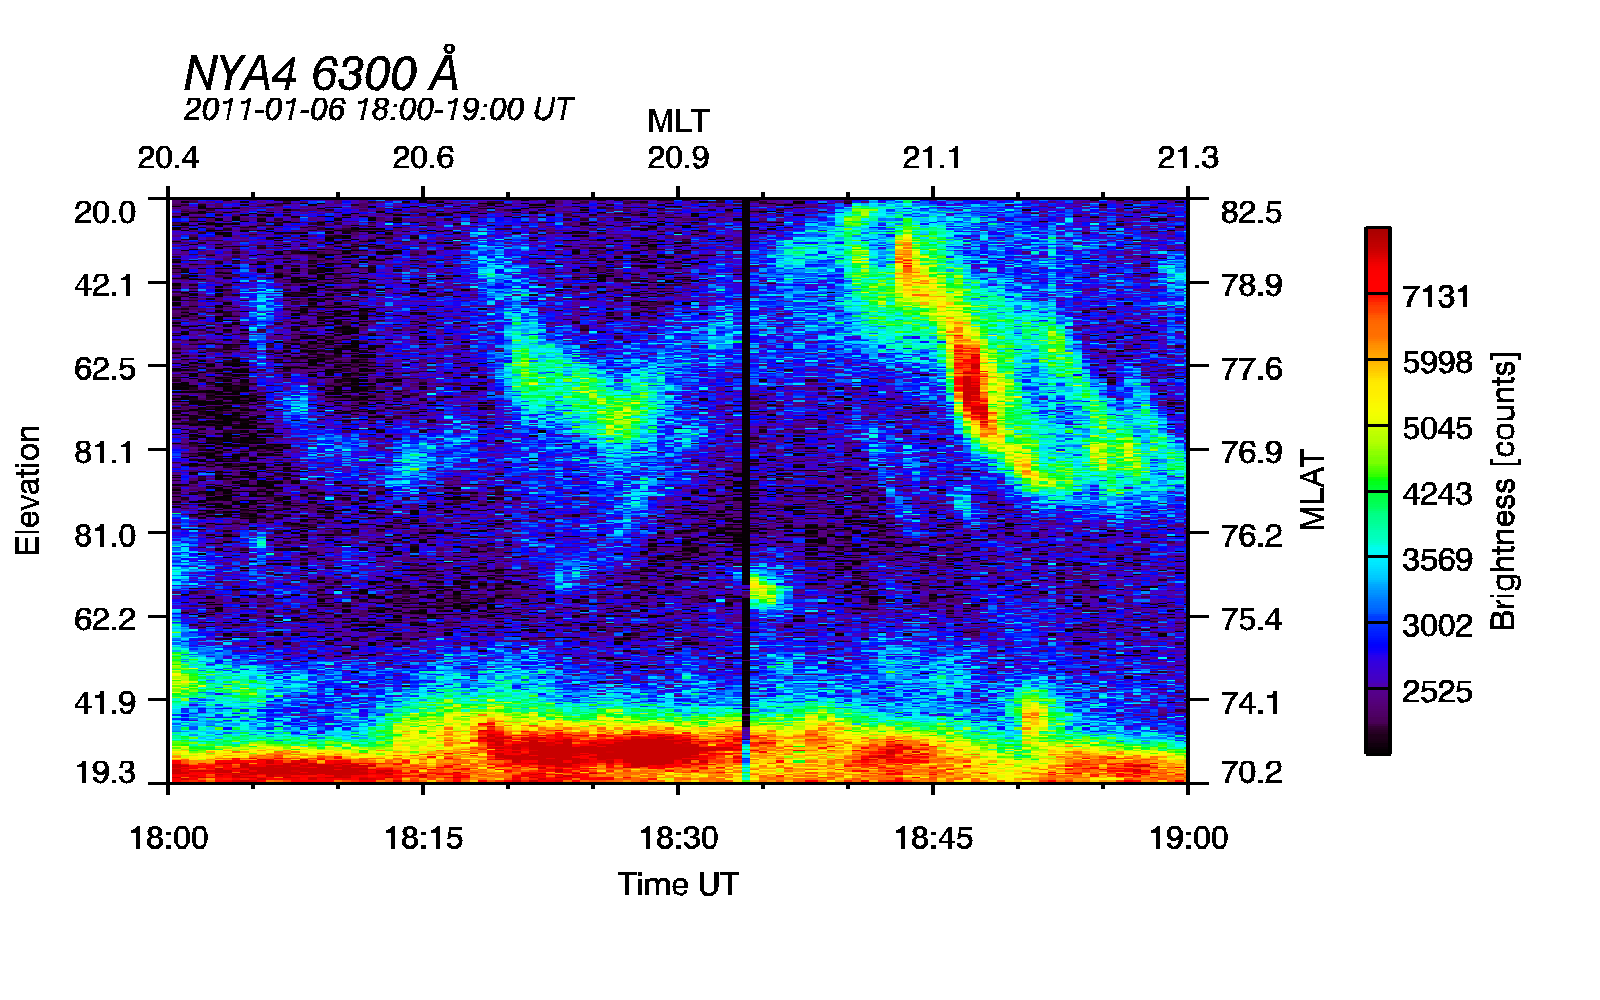
\includegraphics[width=\textwidth]{SvalbardImager6300A18.png}
	\caption{ SvalbardImager at 18:00 o'clock \label{SBI_6_18}}
\end{subfigure}
\begin{subfigure}{0.3\textwidth}
\centering
	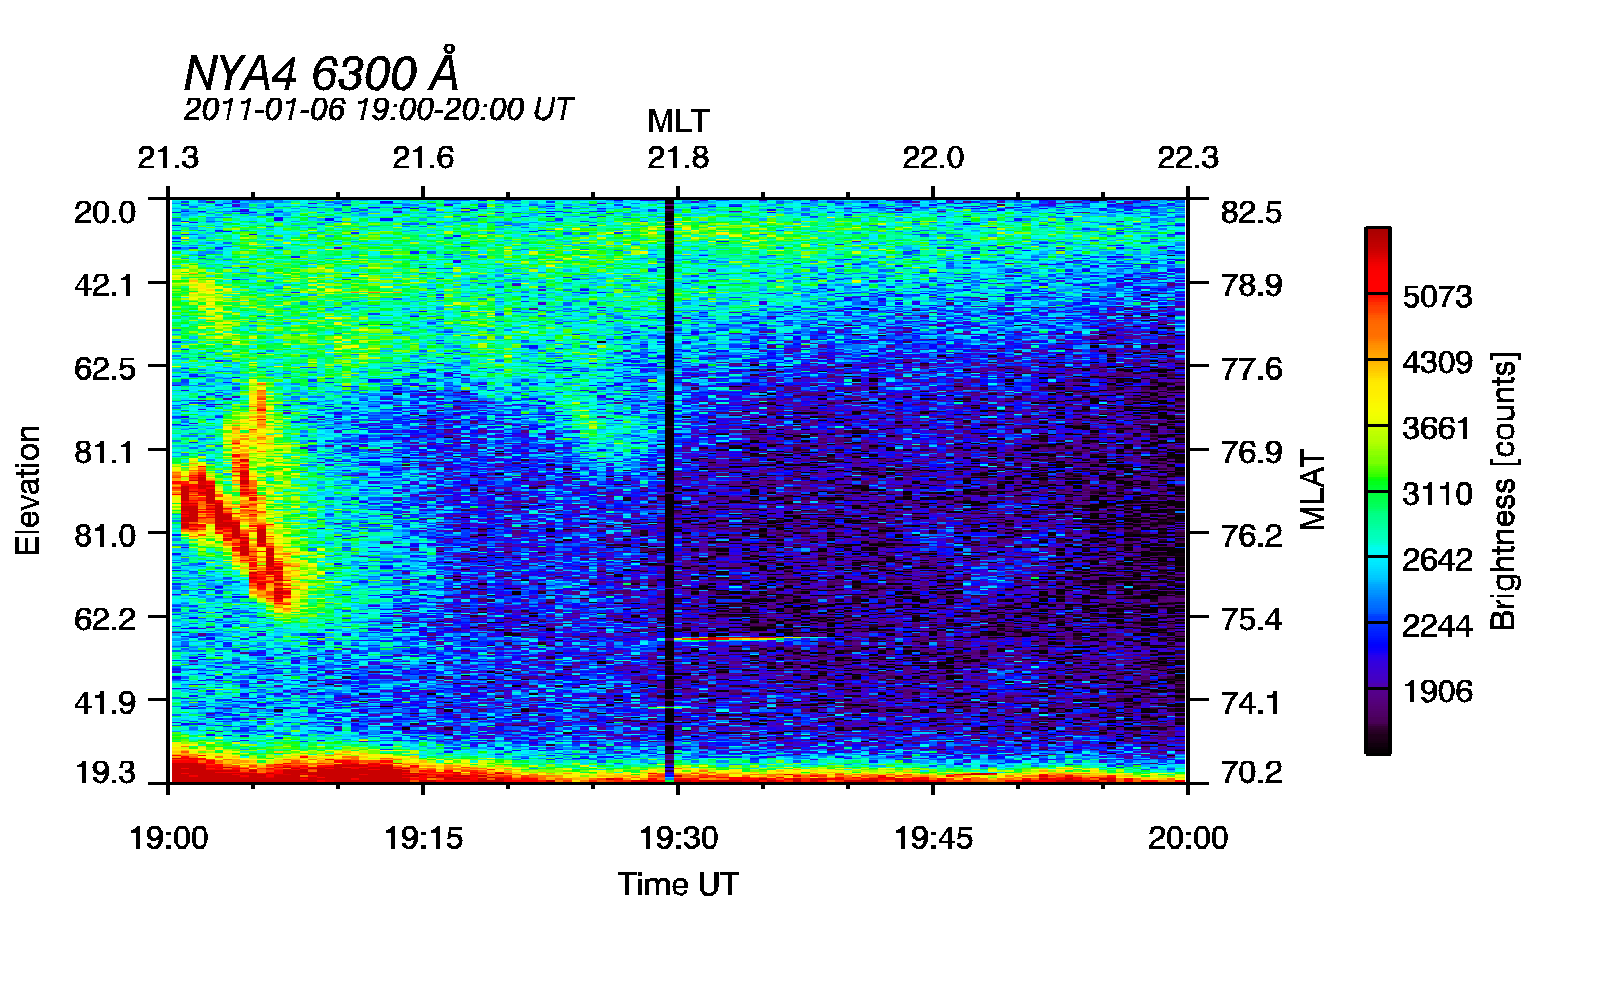
\includegraphics[width=\textwidth]{SvalbardImager6300A19.png}
	\caption{ SvalbardImager at 19:00 o'clock \label{SBI_6_19}}
\end{subfigure}
\begin{subfigure}{0.3\textwidth}
\centering
	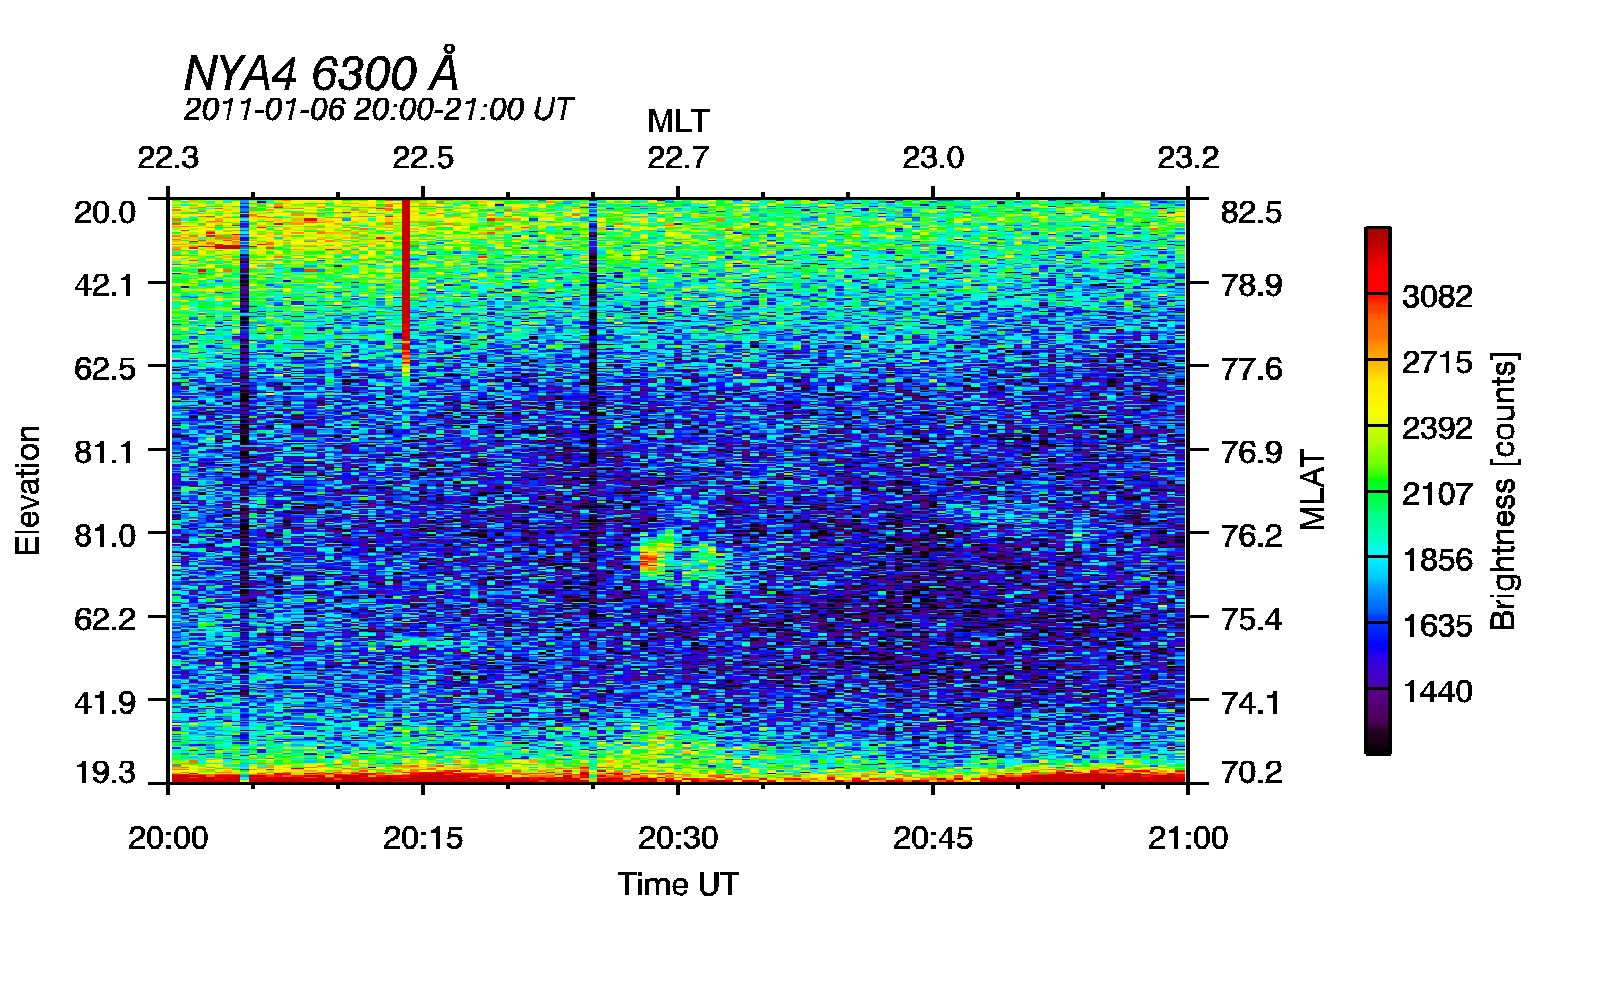
\includegraphics[width=\textwidth]{SvalbardImager6300A20.png}
	\caption{ SvalbardImager at 20:00 o'clock \label{SBI_6_20}}
\end{subfigure}
\begin{subfigure}{0.3\textwidth}
\centering
	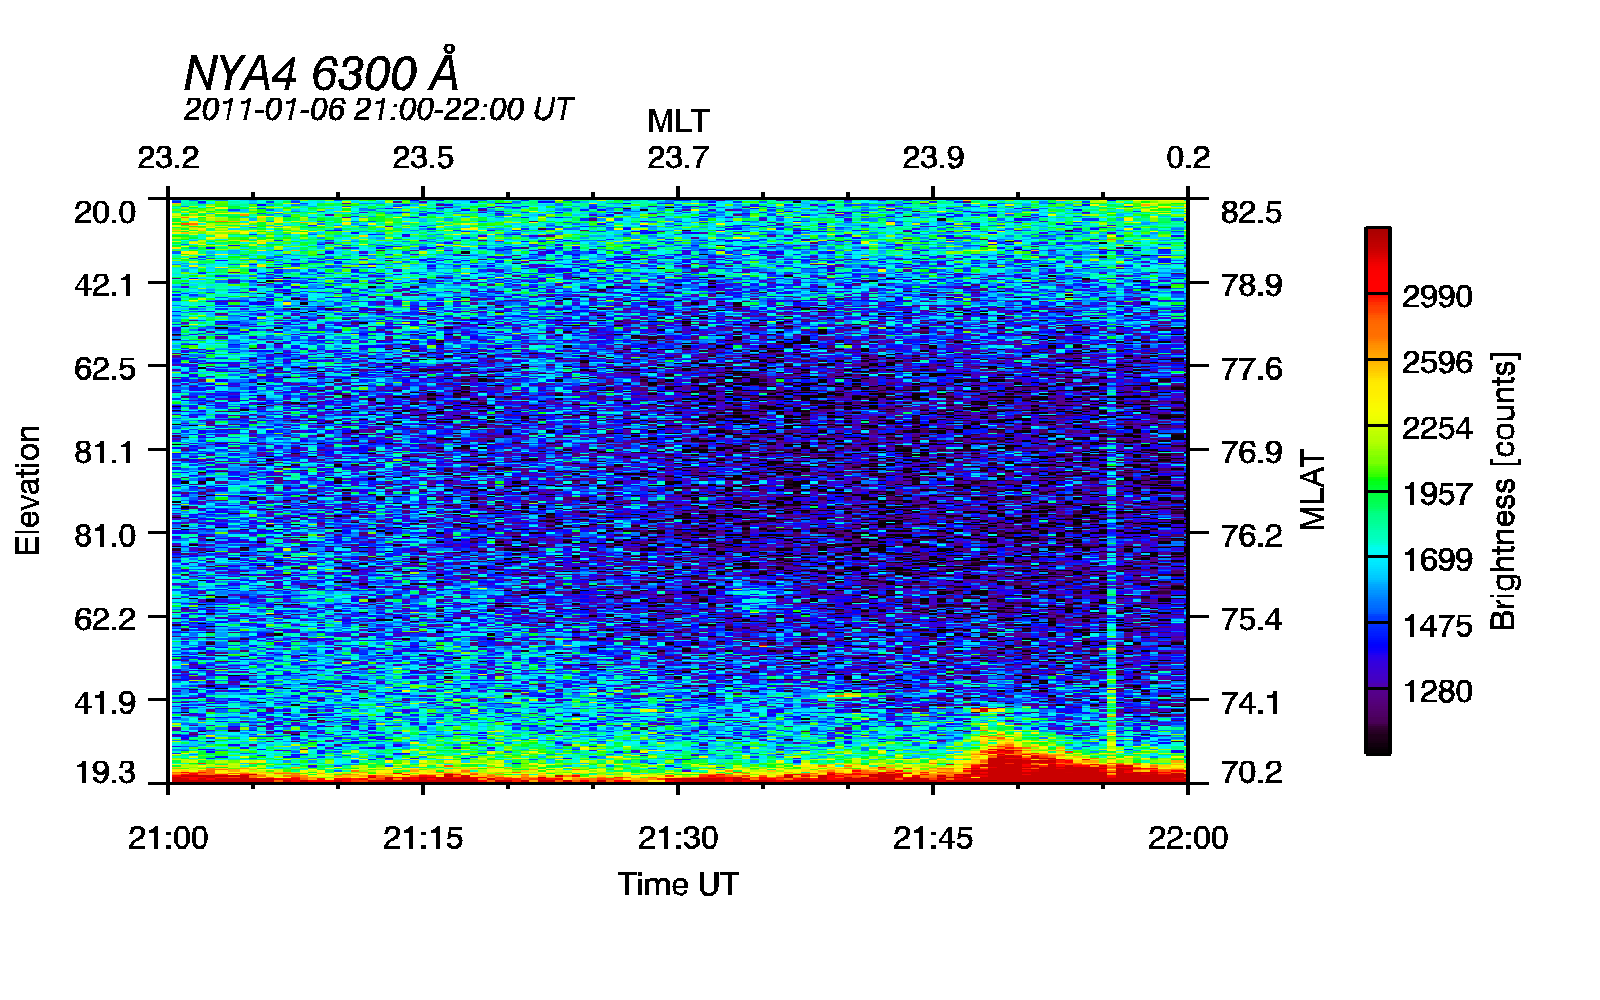
\includegraphics[width=\textwidth]{SvalbardImager6300A21.png}
	\caption{ SvalbardImager at 21:00 o'clock \label{SBI_6_21}}
\end{subfigure}
\begin{subfigure}{0.3\textwidth}
\centering
	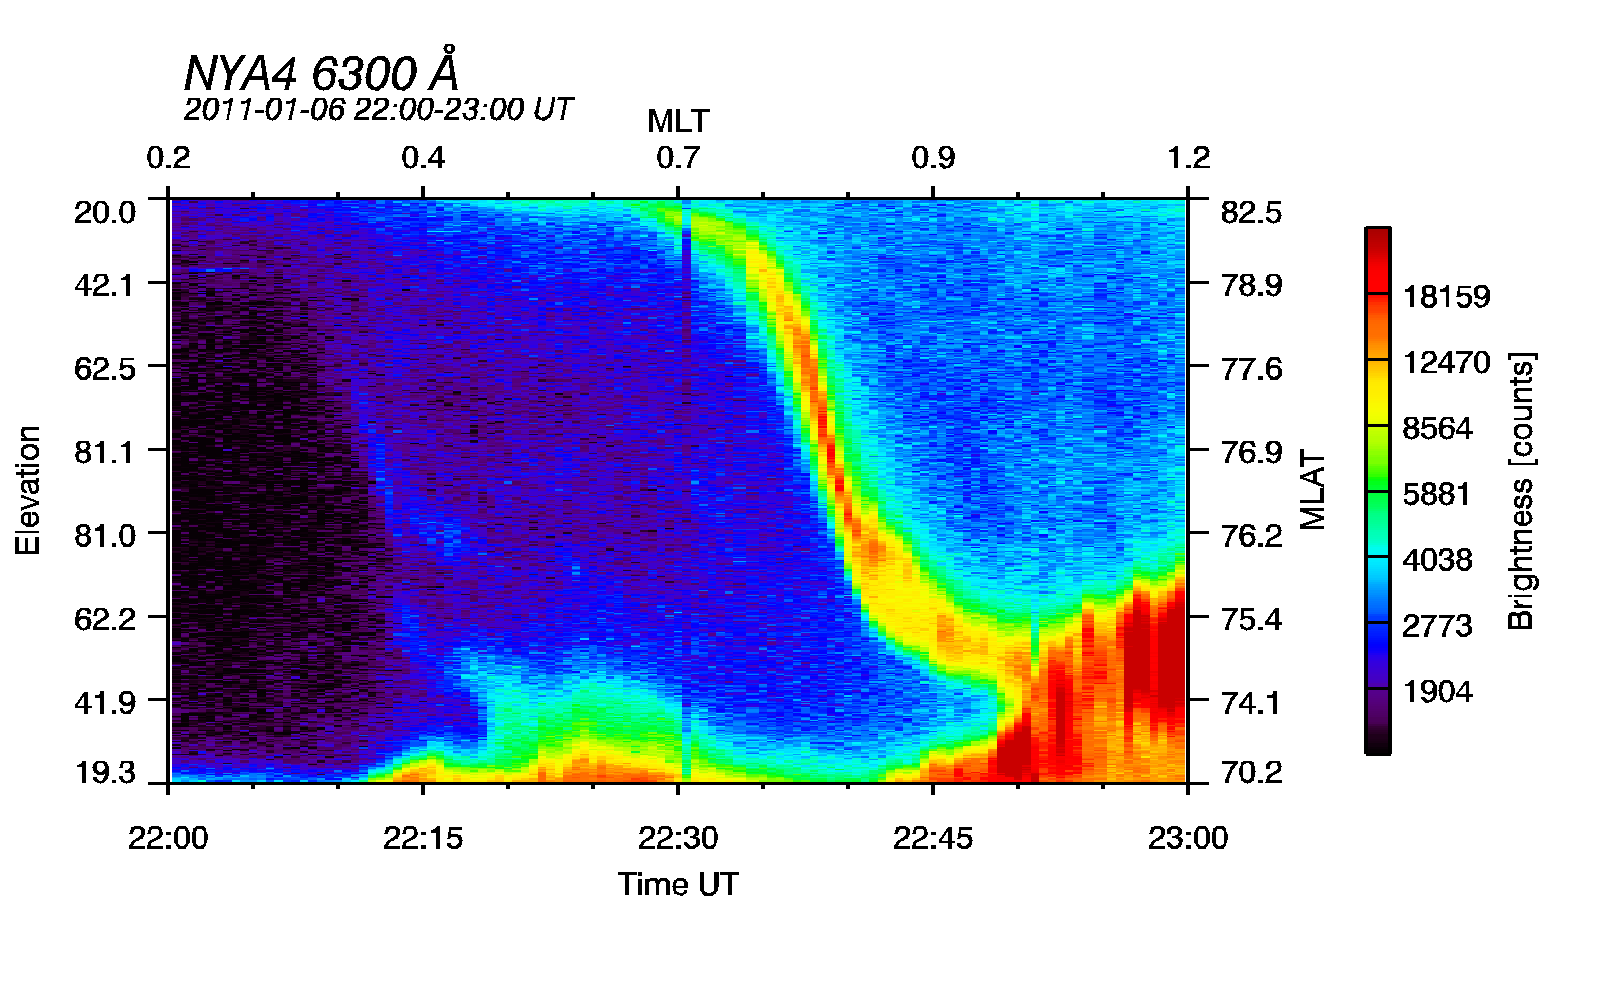
\includegraphics[width=\textwidth]{SvalbardImager6300A22.png}
	\caption{ SvalbardImager at 22:00 o'clock \label{SBI_6_22}}
\end{subfigure}
\begin{subfigure}{0.3\textwidth}
\centering
	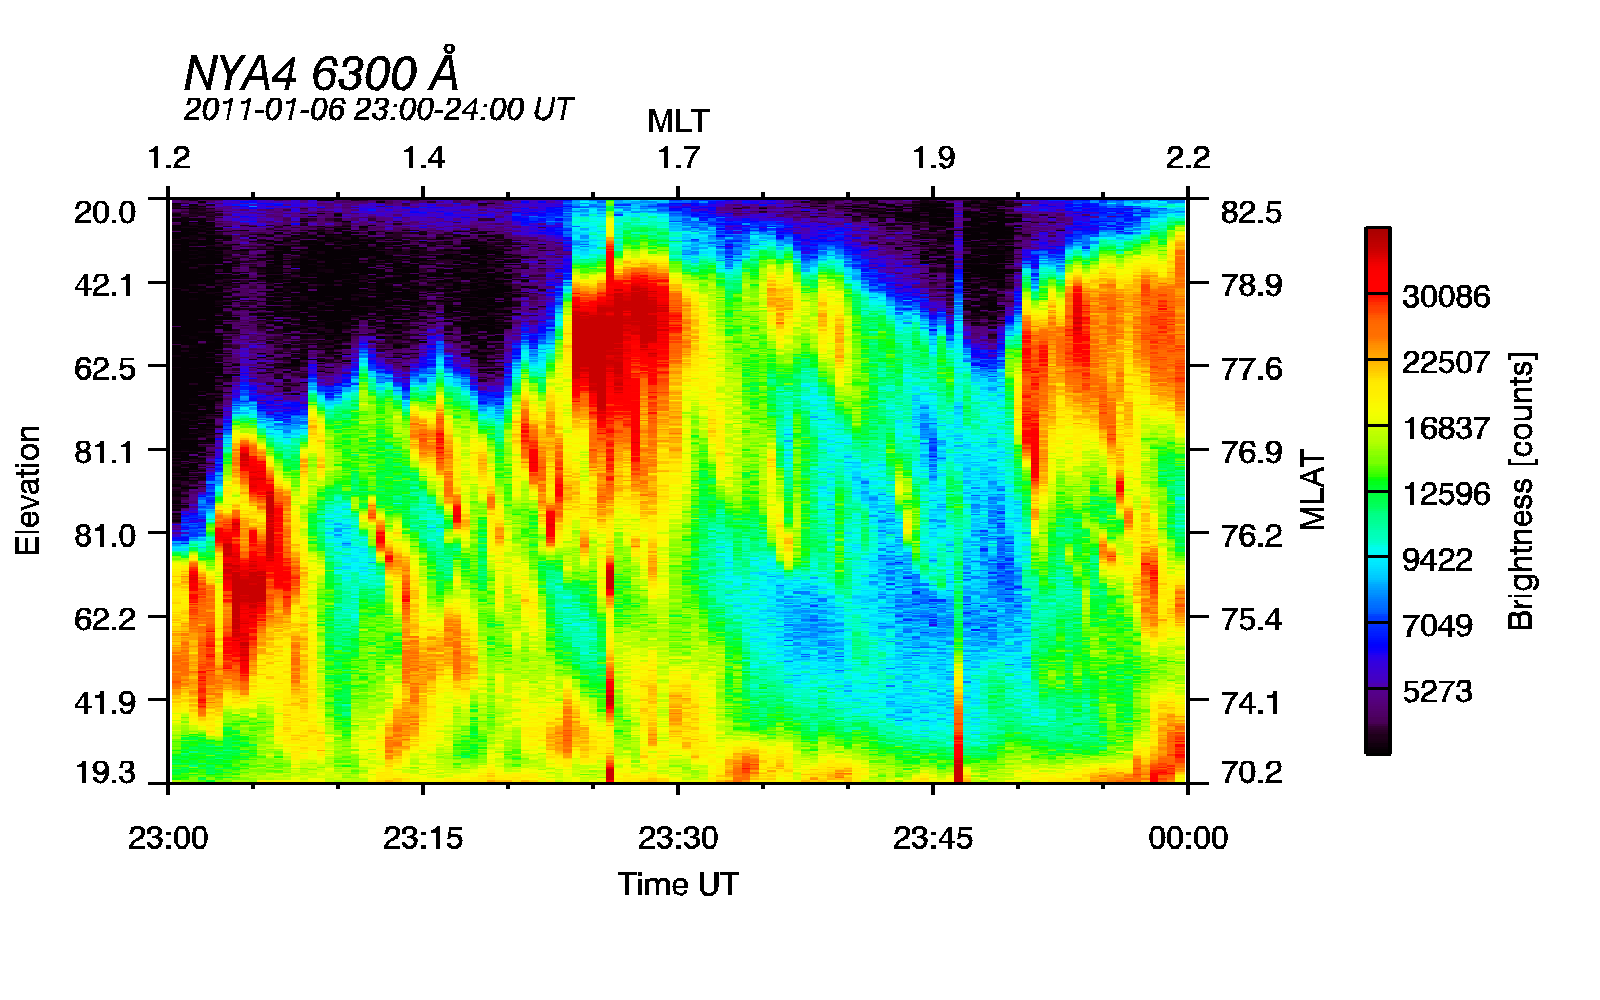
\includegraphics[width=\textwidth]{SvalbardImager6300A23.png}
	\caption{ SvalbardImager at 23:00 o'clock \label{SBI_6_23}}
\end{subfigure}
\caption{Ketograms from the SvalbardImager for $\lambda=6300 \cdot 10^{-10} \mathrm{m}$, different times }
\end{figure}


\clearpage
\section{discussion}

\section{conclusion}


 

\end{document}